\documentclass[10pt,twocolumn,letterpaper]{article}

\usepackage{iccv}
\usepackage{times}
\usepackage{epsfig}
\usepackage{graphicx}
\usepackage{amsmath}
\usepackage{amssymb}
\usepackage[accsupp]{axessibility} 

% User
\usepackage{algorithm}
\usepackage[noend]{algpseudocode}
\usepackage{url}
\usepackage{pgfplots}
\usepackage{tikz}
\usepackage{subcaption}
\usepackage{booktabs}
\usepackage{multirow}
\usepackage{pgfplotstable}
\usepgfplotslibrary{fillbetween}
\usepackage{bbm}
%\usepackage{soul}
\usepackage{anyfontsize}
\usepackage{tabularray}
% \usepackage{titlesec}
% 자간 조정
%\usepackage{microtype}
% Table color
\usepackage{color, colortbl}
\usepackage{float}

\definecolor{cBP}{HTML}{108AE3}
\definecolor{cMF}{HTML}{E3571E}
\definecolor{cdeepBP}{HTML}{1852CC}
\definecolor{cdeepBP8}{HTML}{10AEE3}
\definecolor{cdeepBP32}{HTML}{1CC4DA}
\definecolor{cdeepMF}{HTML}{D62728}
\definecolor{cdeepMF8}{HTML}{ED521F}
\definecolor{cdeepMF32}{HTML}{F69C40}
\definecolor{cMV}{RGB}{44,160,44}
\definecolor{cCL}{HTML}{ED1FD2}
\definecolor{cBayesDGC}{HTML}{A631F5}
\definecolor{Gray}{gray}{0.9}


% \renewcommand{\paragraph}{\smallskip\noindent\textbf}
% \newcommand{\mathbbm}[1]{\text{\usefont{U}{bbm}{m}{n}#1}}
\iffalse
\newenvironment{equationnosep}% environment name 
{% begin code 
  \setlength{\abovedisplayskip}{0pt}%
  \setlength{\belowdisplayskip}{0pt}%
  \setlength{\abovedisplayshortskip}{0pt}%
  \setlength{\belowdisplayshortskip}{0pt}%
  \setlength{\jot}{0pt}%
  \begin{equation}% 
}% 
{\end{equation}}% end code
\fi

\DeclareMathOperator*{\argmax}{arg\,max}
\DeclareMathOperator*{\argmin}{arg\,min}


% Personal color for revision
\newcommand\todo[1]{\textcolor{red}{#1}}
\newcommand{\ok}[1]{{\color{cMF}{#1}}}
\newcommand{\suha}[1]{{\color{cMV}{#1}}}
\newcommand{\khy}[1]{{\color{cBP}{#1}}}
\newcommand{\omh}[1]{{\color{violet}{#1}}}
\newcommand{\hsh}[1]{{\color{cCL}{#1}}}


\newcommand{\set}[1]{\mathcal{#1}}
\newcommand{\kl}{\textnormal{KL}}
\newcommand{\KL}{\textnormal{KL}}


% Include other packages here, before hyperref.

% If you comment hyperref and then uncomment it, you should delete
% egpaper.aux before re-running latex.  (Or just hit 'q' on the first latex
% run, let it finish, and you should be clear).
%\usepackage[pagebackref=true,breaklinks=true,letterpaper=true,colorlinks,bookmarks=false]{hyperref}
\usepackage[pagebackref=true,breaklinks=true,colorlinks,bookmarks=false]{hyperref}

\iccvfinalcopy % *** Uncomment this line for the final submission

\def\iccvPaperID{7270} % *** Enter the ICCV Paper ID here
\def\httilde{\mbox{\tt\raisebox{-.5ex}{\symbol{126}}}}

% Pages are numbered in submission mode, and unnumbered in camera-ready
\ificcvfinal\pagestyle{empty}\fi

\pgfplotsset{compat=1.18}

%\parskip=0.5mm

\begin{document}

%%%%%%%%% TITLE
\title{Adaptive Superpixel for Active Learning in Semantic Segmentation}

% \author{Anonymous submission}

\author{
$\text{Hoyoung Kim}^1$ \quad\quad 
$\text{Minhyeon Oh}^2$ \quad\quad
$\text{Sehyun Hwang}^2$ \quad\quad
$\text{Suha Kwak}^{1,2}$ \quad\quad
$\text{Jungseul Ok}^{1,2} \thanks{Corresponding author.}$\\
\\
$\text{Graduate School of AI, POSTECH}^1$, \quad\quad
$\text{Dept. of CSE, POSTECH}^2$\\
{\tt\small \{cskhy16, minhyeonoh, sehyun03, suha.kwak, jungseul\}@postech.ac.kr}
% Institution1 address\\
% {\tt\small firstauthor@i1.org}
%  minhyeonoh@postech.ac.kr
% For a paper whose authors are all at the same institution,
% omit the following lines up until the closing ``}''.
% Additional authors and addresses can be added with ``\and'',
% just like the second author.
% To save space, use either the email address or home page, not both
}

\maketitle
% Remove page # from the first page of camera-ready.
\ificcvfinal\thispagestyle{empty}\fi



%%%%%%%%% ABSTRACT
\begin{abstract}
Learning semantic segmentation requires pixel-wise annotations, which can be time-consuming and expensive. To reduce the annotation cost, we propose a superpixel-based active learning (AL) framework, which collects a dominant label per superpixel instead. To be specific, it consists of adaptive superpixel and sieving mechanisms, fully dedicated to AL. At each round of AL, we adaptively merge neighboring pixels of similar learned features into superpixels. We then query a selected subset of these superpixels using an acquisition function assuming no uniform superpixel size. This approach is more efficient than existing methods, which rely only on innate features such as RGB color and assume uniform superpixel sizes. Obtaining a dominant label per superpixel drastically reduces annotators' burden as it requires fewer clicks. However, it inevitably introduces noisy annotations due to mismatches between superpixel and ground truth segmentation. To address this issue, we further devise a sieving mechanism that identifies and excludes potentially noisy annotations from learning. Our experiments on both Cityscapes and PASCAL VOC datasets demonstrate the efficacy of adaptive superpixel and sieving mechanisms.


% ==== version 1 ====
\iffalse
Learning-based semantic segmentation requires pixel-wise annotations, which can be time-consuming and expensive. To reduce the annotation cost, we propose a superpixel-based active learning (AL) framework, which collects a dominant label per superpixel instead. To be specific, it consists of adaptive superpixel and sieving mechanisms, fully dedicated to AL. At each round of AL, we adaptively merge neighboring pixels of similar learned features into superpixels. We then query a selected subset of these superpixels using an acquisition function assuming no uniform superpixel size. This approach is more efficient than existing methods, which rely only on innate features such as RGB color and assume uniform superpixel sizes. Obtaining a dominant label per superpixel drastically reduces annotators' burden as it requires fewer clicks. However, it inevitably introduces noisy annotations due to mismatches between superpixel and ground truth segmentation. To address this issue, we further devise a sieving mechanism that identifies and excludes noisy annotations from learning. In our experiments on both Cityscapes and PASCAL VOC datasets, we demonstrate the efficacy of adaptive superpixel and sieving mechanisms.
\fi


%\vspace{7cm}
% Active learning selectively obtains labels for the most informative samples, which can achieve comparable performance with full supervision while reducing the time and cost of annotations.
% Region-based are shown to offer better performance than whole image sampling, however, under realistic click-based annotations costs, region size becomes an important consideration.
% Superpixels can facilitate labeling by grouping surrounding pixels into perceptually meaningful regions, but their over-segmentation and size can lead to higher labeling costs and lower-quality dominant labels. To address this, the authors propose an adaptive approach to updating the pool of superpixels by merging multiple superpixels into one based on a model that is updated after each round and introducing a new evaluation metric based on achievable segmentation accuracy.

% Active learning selectively obtains labels for the most informative samples, which can achieve comparable performance with full supervision while reducing the time and cost of annotations.
% In active learning for semantic segmentation, superpixels, which group surrounding pixels into perceptually meaningful regions, have been shown to be more efficient in reducing click-based annotation costs compared to using rectangles. 
% However, the over-segmentation of superpixels can result in higher labeling costs for large regions. 
% To address this, we propose an adaptive approach to update the pool of superpixels by merging multiple superpixels based on a model that is updated after each round. Furthermore, we introduce a superpixel-wise denoising technique and a new evaluation metric for merged superpixels. 
% The results demonstrate that the proposed method achieves high segmentation accuracy while reducing annotation costs, making it a promising approach for active learning in semantic segmentation.
\end{abstract}

%%%%%%%%% BODY TEXT

\let\hl=\undefined
\newcommand\hl[1]{\textcolor{blue}{#1}}

\begin{figure}[!t]
    % \captionsetup[subfigure]{font=footnotesize}
    \centering
    \begin{subfigure}[h!]{.49\linewidth}
        \centering
        % \includegraphics[scale=0.078]{Figures/aachen_000000_000019.jpg}
        \includegraphics[scale=0.231]{Figures/fig1/fig_1_a.png}
        % \includegraphics[scale=0.121]{Figures/fig1/fig1_a.png}
        \caption{Over-segmented $(t=0)$}
        \label{(a)-adaptive}
        \vspace{2mm}
    \end{subfigure}
    \begin{subfigure}[h!]{.49\linewidth}
        \centering
        % \includegraphics[scale=0.078]{Figures/cityscapes_merged_round1.jpg}
        \includegraphics[scale=0.231]{Figures/fig1/fig_1_b_v2.png}
        % \includegraphics[scale=0.121]{Figures/fig1/fig1_b.png}
        \caption{Adaptive merged $(t=2)$}
        \label{(b)-adaptive}
        \vspace{2mm}
    \end{subfigure}
    \begin{subfigure}[h!]{.49\linewidth}
        \centering
        % \includegraphics[scale=0.078]{Figures/cityscapes_merged_round1.jpg}
        \includegraphics[scale=0.231]{Figures/fig1/fig_1_c_v2.png}
        % \includegraphics[scale=0.121]{Figures/fig1/fig1_c.png}
        \caption{Adaptive merged $(t=4)$}
        \label{(c)-adaptive}
    \end{subfigure}
    \begin{subfigure}[h!]{.49\linewidth}
        \centering
        % \includegraphics[scale=0.078]{Figures/cityscapes_merged_round1.jpg}
        \includegraphics[scale=0.231]{Figures/fig1/fig_1_d_v4.jpg}
        % \includegraphics[scale=0.121]{Figures/fig1/fig1_d.png}
        \caption{Oracle}
        \label{fig:(d)_adaptive_merged_superpixels}
    \end{subfigure}
    \caption{{\em Examples of adaptive superpixels.} (a) We begin active learning with over-segmented superpixels. (b, c) In each round $t$, we merge superpixels in an adaptive manner using the model from the previous round. % $t-1$. 
    (d) As the round progresses, adaptive superpixels look similar to oracle ones.}
    \label{fig:adaptive_merged_superpixels}
    % \vspace{-3mm}
\end{figure}

\begin{figure*}[t!]
    \centering
    \includegraphics[scale=0.52]{Figures/overall_arch_share_v7.pdf}
    \caption{{\em An overview of the proposed framework.} In each round $t$, we merge superpixels with a graph using the latest model, and obtain dominant labels for selected superpixels. The dominant labels are selectively propagated to pixels with confidence above the detected knee point, resulting in the creation of a sieved dataset. Finally, we train a model with the sieved one.}
    \label{fig:method}
    % \vspace{-2mm}
\end{figure*}

\section{Introduction}
With the advent of deep learning, many computer vision tasks including semantic segmentation have dramatically evolved in recent years.
Such advances are thanks to complex deep network models that can learn huge datasets. However, labeling such large datasets is prohibitively time-consuming and labor-intensive, in particular, for semantic segmentation tasks that demand a dense annotation on each pixel \cite{Cordts2016Cityscapes, everingham2015pascal}. Active learning (AL) offers an approach to alleviate the annotation cost  by selectively querying only the most informative samples to annotators.

%selectively obtaining labels for the most informative pixels determined by a well-designed acquisition function.
%In general, the acquisition function prioritizes the selection of unlabeled samples that a model is uncertain about, in order to improve the performance.
% =====
% what is efficient query?
% reviisiting
% =====

Designing an effective form of annotation query is critical in practice 
as it determines the actual annotation cost such as the number of clicks required
and the informativeness per annotation query.
For semantic segmentation, an image-wise query can be asked for a complete annotation on the semantic of every pixel in an image~\cite{chengliang2020suggestive,desai2022active,sinha2019variational,xie2020deal,yang2017suggestive}.
This is a daunting task requiring an enormous amount of clicks to indicate boundaries (using polygons or contours) for each semantic segment or to annotate semantic pixel-wisely, while 
the diversity of contexts which we can observe in a single image is restricted. 
Alternatively, one can design a {\it region-based}
query enquiring only about the dominant label of a small region such as rectangle patch \cite{casanova2019reinforced,qiao2022cpral,xie2022towards} or superpixel 
%(a cluster of neighboring superpixels of similar color )
\cite{cai2021revisiting,siddiqui2020viewal}. 
This is known to be simple yet effective 
as it requires only a single click per query while enabling AL to put more focus on significant regions
and to avoid annotation wastes.

% partition an image into multiple regions and request each region as a query~\cite{qiao2022cpral,mackowiak2018cereals,casanova2019reinforced,siddiqui2020viewal}. 
%This way is often useful since learning procedure can put more focus on important regions avoiding waste of annotation effort.
% Additionally, the labeling mechanism can be further optimized based on the shape of regions.
% Also, based on the shape of regions, labeling mechanism can be further optimized. 
% With rectangular partitioning, a sparse set of clicks (\ie., polygon vertices on the segmentation contour and class assignment) can recover dense pixel-wise annotations for each patch~\cite{colling2020metabox+,mackowiak2018cereals}.
% With boundary-preserving partitioning (\eg., superpixels), only one click is sufficient for labeling each queried region
% ~\cite{cai2021revisiting} since answering the majority class of pixels within each region is enough. 
% We refer to that label obtained in that way as the dominant label.


\iffalse
In AL for semantic segmentation, it is possible to request dense pixel-wise annotation~\cite{casanova2019reinforced,qiao2022cpral,yang2017suggestive} 
%to an oracle who always provides correct labels, 
while it makes the annotation process daunting due to the direct proportionality between the required number of clicks and the query's granularity (\eg., images or regions).
Instead, one can partition each unlabeled image into boundary-preserving pixel groups (\ie., superpixels), and request labels for them.
Using superpixels as the units for querying allows for efficient labeling, as only one click is needed to label each queried superpixel~\cite{cai2021revisiting}. This is due to the fact that determining the majority class of pixels within a superpixel is sufficient for labeling purposes. We refer to a label obtained by the majority click as the dominant label.
\fi

%However, under realistic click-based annotation costs~\cite{cai2021revisiting,colling2020metabox+,mackowiak2018cereals}, the oracle should click in proportion to the number of pixels in the patches, which causes increased costs as the patch size increases.
%The leverage of superpixels in AL facilitates the labeling of one semantic category per region with a click by grouping neighboring pixels into perceptually meaningful regions~\cite{cai2021revisiting, siddiqui2020viewal}.
%The annotation of a superpixel is conducted by obtaining the majority class of pixels within the superpixel, known as dominant labeling.
%Recent research demonstrates that using superpixels reduces the click budgets compared to using rectangles~\cite{cai2021revisiting}.


\iffalse
In the context of AL for semantic segmentation, there exist two query granularities: rectangle and superpixel units. 
% In AL for semantic segmentation, granularity of query is typically two-kinds: image-level, or regional units. 
Using each image as a query~\cite{chengliang2020suggestive,desai2022active,sinha2019variational,xie2020deal,yang2017suggestive} requires annotators to assign semantic categories to each pixel in the entire image, leading to a high annotation burden.
Alternatively, one can partition an image into multiple regions and request each region as a query~\cite{qiao2022cpral,mackowiak2018cereals,casanova2019reinforced,siddiqui2020viewal}. 
%This way is often useful since learning procedure can put more focus on important regions avoiding waste of annotation effort.
This approach is frequently beneficial as AL can put more focus on significant regions, avoiding wasting annotation effort.
% preventing unnecessary annotation efforts from being wasted.
Additionally, the labeling mechanism can be further optimized based on the shape of regions.
% Also, based on the shape of regions, labeling mechanism can be further optimized. 
With rectangular partitioning, a sparse set of clicks (\ie., polygon vertices on the segmentation contour and class assignment) can recover dense pixel-wise annotations for each patch~\cite{mackowiak2018cereals,colling2020metabox+}.
With boundary-preserving partitioning (\eg., superpixels), only one click is sufficient for labeling each queried region
~\cite{cai2021revisiting} since answering the majority class of pixels within each region is enough. 
We refer to that label obtained in that way as the dominant label.
\fi

\iffalse
Pixel-wise annotations are obtained for the most informative patches with the help of an oracle who always provides correct labels.
However, under realistic click-based annotation costs~\cite{cai2021revisiting,colling2020metabox+,mackowiak2018cereals}, the oracle should click in proportion to the number of pixels in the patches, which causes increased costs as the patch size increases.
The leverage of superpixels in AL facilitates the labeling of one semantic category per region with a click by grouping neighboring pixels into perceptually meaningful regions~\cite{cai2021revisiting, siddiqui2020viewal}.
The annotation of a superpixel is conducted by obtaining the majority class of pixels within the superpixel, known as dominant labeling.
Recent research demonstrates that using superpixels reduces the click budgets compared to using rectangles~\cite{cai2021revisiting}.
\fi

% ^~~ dominant labeling
% ^~~ polygon clicks, intersection clicks, etc.
% =====
% oversegmentation, throuput problem
% =====


AL with the region-based query needs a delicate generation of candidate regions to be queried. A small region size dilutes the budget efficiency, whereas the dominant labeling even by a perfect annotator is prone to give noisy labels when regions are too large to be consisting of pixels with a single class. However, the previous works~\cite{casanova2019reinforced,qiao2022cpral,siddiqui2020viewal}
rely on a fixed candidate set of regions of uniform size, while we could adjust the size and shape of candidate regions as we train the semantic segmentation model over rounds of AL. This limitation remains even in recent work \cite{cai2021revisiting}
with superpixel candidates providing less 
risk of noisy labels than rectangle ones
since the superpixels are produced, only at the beginning, by a conventional superpixel algorithm,
where conventional superpixel algorithms ~\cite{achanta2012slic,jianbo2000normalized,van2012seeds} cluster adjacent pixels of similar innate features (\eg., color) with implicit or explicit regularization to make similar sizes or shapes of superpixels, \ie., limited freedom of query region.



%\vspace{-.4mm}

\let\oldparskip=\parskip
\parskip=0mm

In this paper, to fully enjoy the benefit in terms of annotation cost while suppressing the risk of noisy labels, 
we devise an AL framework, illustrated in Figure~\ref{fig:method}, consisting of adaptive merging and sieving methods.
The adaptive merging method % (Figure~\ref{fig:method})
repeatedly evolves the candidate superpixels for dominant labeling at every round with the latest model and no explicit regularization on the size and shape of superpixels.
% we propose an adaptive merging algorithm~(Figure~\ref{fig:method}) that aims to increase labeling efficiency by merging adjacent and similar superpixels using a trained model. 
This indeed enables the continual improvement 
of
the superpixels' ability to accurately capture the boundaries of semantic objects~(Figure~\ref{(b)-adaptive} and \ref{(c)-adaptive}),
and a proper variation in the sizes and shapes of superpixels, \ie., larger superpixels being attached to larger semantic objects (\eg., road and building) and smaller ones to smaller objects (\eg., human and vehicle) as shown in the ideal ones~(Figure~\ref{fig:(d)_adaptive_merged_superpixels}).


% where the former
% evolves the candidate superpixels for dominant labeling at every round,
% and the latter identifies and leaves out annotations with the high risk of noisy labels given the latest model.

% In the merging process, superpixels with different dominant labels may be merged, and even if superpixels are merged accurately, noisy labels can exist due to the inherent imperfectness of superpixels.
% As the dominant label of a superpixel propagates to its constituent pixels, the ground-truth of a pixel and the dominant label can differ.

Given the adaptive superpixels, we establish
a corresponding acquisition function being aware of irregular superpixel sizes.
It prioritizes uncertain superpixels of rare classes
in order to query the most informative superpixels while balancing class distributions in the entire annotations. In addition, 
to alleviate the inevitable noise in the dominant labeling, we propose a sieving technique 
that excludes labeled pixels of high potential risks of being different classes than the dominant one. 
To be specific, we identify such pixels of potentially noisy labels by 
per-superpixel sieving with distinct thresholds over superpixels. This provides stabler denoising 
than uniform sieving with a constant threshold, which might aggravate class imbalance in the sieved annotations. 
%the  provides class imbalance.

%relatively unsure pixels within each queried superpixel from training. 
%The remaining labeled areas are then utilized for training the model.
%Here, the per-superpixel sieving provides class imbalance.

% prevents class imbalance 
% since the noise is recognized using a distinct threshold for each superpixel.

\parskip=\oldparskip

\iffalse
The adoption of superpixel-wise dominant labeling in AL for semantic segmentation significantly reduces the annotation burden~\cite{cai2021revisiting}.
However, conventional algorithms for superpixel generation~\cite{achanta2012slic,jianbo2000normalized,van2012seeds} are unsuitable for AL. 
This is because superpixels are designed for over-segmenting images into regions that are regular in shape and size~\cite{levinshtein2009turbopixels} (Figure~\ref{(a)-adaptive}), which can constrain the formation of more effective queries.
Since the throughput of every query is bounded by the number of pixels in the smallest semantic area in the dataset, it is necessary to discard the regularity constraints from the process of superpixel generation in order to reflect the actual size of semantic objects in the dataset. 
%Moreover, the size of superpixels significantly influences the quality of partitioning, which in turn affects the performance of AL.
%From a perspective of labeling efficacy, diverse size of superpixels reflecting the actual size of objects is necessary.
% However, determining the optimal superpixel size in advance of AL rounds is a challenging task.



In order to fully enjoy the benefits of dominant labels, we propose an adaptive approach that updates the base superpixels by merging adjacent and similar superpixels into a single one per round, based on a model trained in the previous round~(Figure~\ref{fig:method}).
% we propose an adaptive merging algorithm~(Figure~\ref{fig:method}) that aims to increase labeling efficiency by merging adjacent and similar superpixels using a trained model. 
Additionally, we repeatedly perform such consolidation in an adaptive manner to improve the superpixels' ability to accurately capture the boundaries of semantic objects~(Figure~\ref{(b)-adaptive} and \ref{(c)-adaptive}). 
This approach results in a variation in the sizes of superpixels, with larger superpixels being attached to larger semantic objects (\eg., road and building) and smaller ones to smaller objects (\eg., human and vehicle). 
By repeating the adaptive merging at each round, superpixels become more similar to the ideal ones~(Figure~\ref{fig:(d)_adaptive_merged_superpixels}).

% Superpixel-wise dominant labeling dramatically reduce annotation burden in AL for segmentation,
% however, conventional superpixel generation algorithms
% Also, choice of the common size of superpixels hugely affects the quality of partitioning \cite{goh2021sizes}, which in turn affects the performance in AL. 
% However, it is difficult
% (or even impossible), in practice, 
% to find the best choice of superpixel size in advance of AL rounds. 
% for active semantic segmentation
% ^~~~ 좀 더 명확한 문장으로
% static 관련 얘기 들어가야됨
% =====
% importance of "adaptive" "merging"
% =====
%To fully enjoy dominant labeling, our motivation is two-fold: removing uniformity in superpixel size, by merging them with the aid of a trained model, can make labeling more efficient (Figure~\ref{(b)-adaptive}); and adaptively repeating such consolidation can make superpixels align with the ideal ones (Figure~\ref{(c)-adaptive} and \ref{fig:(d)_adaptive_merged_superpixels}). 
%To fully enjoy the dominant labeling, our objective is two-fold: to remove uniformity in superpixel size, by merging them with the aid of a trained model, to make labeling more efficient (Figure~\ref{(b)-adaptive}); and to adaptively repeate such consolidation to make superpixels better capture the boundaries of ideal superpixels (Figure~\ref{(c)-adaptive} and \ref{fig:(d)_adaptive_merged_superpixels}).
%\todo{In order to fully utilize the dominant labeling, our objective is two-fold. Firstly, to increase labeling efficiency, we aim to eliminate uniformity in superpixel size by merging them with the assistance of a trained model~(Figure~\ref{(b)-adaptive}). Secondly, we aim to repeatedly perform this consolidation in an adaptive manner, thereby enhancing the ability of the superpixels to accurately capture the boundaries of ideal superpixels~(Figure~\ref{(c)-adaptive} and \ref{fig:(d)_adaptive_merged_superpixels}). With this approach, size of superpixels becomes varied in a way that lager superpixels are attached to larger semantic objects (\eg., road and building) and smaller ones to smaller objects (\eg., human and vehicle).}
% [More details here?]
% By repeating the adaptive merging at each round, we can achieve superpixels that closely resemble the ideal ones~(Figure~\ref{fig:(d)_adaptive_merged_superpixels}).
%our objective is two-fold. Firstly, to increase labeling efficiency, we aim to eliminate uniformity in superpixel size by merging them with the assistance of a trained model~(Figure~\ref{(b)-adaptive}). Secondly, we aim to repeatedly perform this consolidation in an adaptive manner, thereby enhancing the ability of the superpixels to accurately capture the boundaries of ideal superpixels~(Figure~\ref{(c)-adaptive} and \ref{fig:(d)_adaptive_merged_superpixels}).


% =====
% noise, how to?
% =====

%The merging procedure seems efficient, though merged superpixels may contain severe noise that degrades model performance. 
%The merging procedure could save annotation budget, while merged superpixels may contain noise that degrades model performance.
In the merging process, superpixels with different dominant labels may be merged, and even if superpixels are merged accurately, noisy labels can exist due to the inherent imperfectness of superpixels.
As the dominant label of a superpixel propagates to its constituent pixels, the ground-truth of a pixel and the dominant label can differ.
To alleviate the side effect of noisy labels, we propose a sieving technique~(Figure~\ref{fig:method}) 
that identifies less certain areas within each labeled superpixel and eliminates them. 
The remaining labeled areas are then utilized for training the model.
This denoising approach prevents class imbalance 
% and preserves region diversity 
since the noise is recognized using a distinct threshold for each superpixel.
\fi
% By denoising the labels in this manner, we can prevent class imbalance and remain region diversity since the noise is detected using different criteria for each superpixel.
% that only uses the annotation on pixels with high confidence to the dominant label.
% The merging process can help to save annotation cost, but it may introduce noise into the merged superpixels, which can degrades the performance of the model.
%Such noise occurs when superpixels with different majority classes are merged, which can be frequent at early rounds due to model instability; or is retained when over-segmented base superpixels, generated before active learning starts, fail to preserve the exact boundary of semantic objects. 
% This type of noise arises when superpixels with distinct majority classes are combined, which can be common during the early rounds due to the instability of the model,
% or when over-segmented base superpixels, produced prior to active learning, fail to preserve the exact boundaries of semantic objects.
% TOO LONG...
%To mitigate the effect of noise, we propose an adaptive sieving technique that detects less-confident parts for each of the labeled superpixels, and throws such parts away from them. 
% To reduce the impact of noise, we propose an adaptive sieving technique~(Figure~\ref{fig:method}) that identifies less confident areas within each labeled superpixels and eliminates them. The remaining labeled areas are then fed into the model for training.
%Denoising labels in such a way can avoid class imbalance since noise is detected with different criteria for different superpixels, and gradually improves as the rounds proceed.
% By denoising the labels in this manner, we can prevent class imbalance since the noise is detected using different criteria for each superpixel.
% , and gradually improves as the rounds progress.

% =====
% performance improvements
% 8192 > 512
% (intution, justification) new metric -> look-ahead performance -> (inspection) choice of base superpixel
% =====

Through the integration of adaptive merging and sieving into an AL framework, we achieve improved 
accuracy and budget-efficiency over a baseline method. 
% that relies solely on the dominant labels of superpixels.
% Notably, the merging is effective under small superpixels and the sieving is effective under large superpixels, which is related to the qunantity and quality of labels, respectively.
Notably, the merging demonstrates effectiveness under small-sized superpixels, while the sieving plays a critical role given large-sized superpixels.
%which are associated with the quantity and quality of labels, respectively.
Moreover, we show a consistent improvement 
over existing methods in various settings. %independent of the base size.
% Notably, the benefits are apparent when the size of base superpixels is small. 
% as the merging of adjacent and similar superpixels becomes more effective.
% In addition, we show a consistent improvement independent of the base size.
% minimal performance guarantee that is invariant to the choice of the base size.
We provide a thorough justification of the proposed method using various quantitative measures, 
where we introduce 
a new evaluation metric for superpixel algorithms 
that assesses both (achievable) accuracy and recall,
where the recall is overlooked in 
the existing one, the achievable segmentation accuracy~(ASA)~\cite{liu2011entropy}
but important in the context of AL.
This may give new insights into developing superpixel algorithms.
% This may give a new insight 
% being aware of annotation cost and 
% in the context
% of AL, while ,
% irrespective of 
% which assesses the quality of labels,
% % the consistency within a superpixel
% and a modified version of the ASA metric, which enables us to also assess the quantity of labels.
\iffalse
We thoroughly inspect
\fi

% the look-ahead performance of the superpixels.

% consistent improve
% We also introduce a modified version of ASA, specifically designed to evaluate superpixels in the context of our proposed framework.
% We demonstrate improved performance over a baseline method, which utilizes only static superpixels and dominant labeling, by incorporating adaptive merging and sieving into the active learning framework. The benefits are particularly noticeable when the size of the base superpixels is small, as the merging of adjacent and similar superpixels becomes more effective.
% Also, we show minimal guarantee on performance boost which is invariant to the choice of the base size.
%Furthermore, we provide a minimal performance boost guarantee that is independent of the choice of the base size.
%In addition, to explain such advancement, we inspect superpixels with various quantitative measures: achievable semantic segmentation~(ASA)~\cite{liu2011entropy} which evaluates consistency within a superpixel; and achievable precision~(AP), recall~(AR) and F1-score~(AF) which are introduced to take into account both quality and throughput since the need for reflecting superpixel size is brought about by the merging algorithm.
% To analyze such advancement, we inspect superpixels using various quantitative measures, including the achievable semantic segmentation~(ASA)~\cite{liu2011entropy} which assesses the consistency within a superpixel. 
% We also introduce a modified version of ASA, specifically designed to evaluate superpixels in the context of our proposed framework.
% \todo{In addition, we propose new evaluation metrics for superpixels, which are more suitable under the proposed framework.
% Conventionally, superpixels are evaluated by the consistency and boundary alignment within a superpixel \cite{achanta2012slic,jampani2018superpixel,yang2020superpixel}, both of which focus on the quality of superpixels. 
% However, the need for reflecting superpixel size is brought about by the merging algorithm. 
% Therefore, we suggest quantitative metric based on F1-score, taking into account both the quality and throughput.
% Furthermore, we show high correlation between the metric and AL performance, thereby providing an effective tool to look-ahead consequence of base superpixel selection.}

Our main contributions are summarized as follows:
\begin{itemize}
    \item We propose an adaptive merging algorithm where superpixels are updated at each round (Section~\ref{sec:adaptive-merging}), and show the effectiveness of adaptive merging rather than only merging once (Section~\ref{sec:effect-of-adaptive}).
    \item We alleviate the side effect of noisy labels via a sieving technique (Section~\ref{sec:sieving-technique}), and demonstrate especially efficient under large superpixels (Section~\ref{sec:effect-of-adaptive}).
    \item
    In various realistic experiments, we demonstrate the consistent improvement of the proposed AL framework, consisting of the adaptive merging and sieving methods with the dedicated acquisition function, over existing ones (Section~\ref{sec:effect-of-adaptive}).
    \item
    We provide an insightful analysis on proper superpixels for AL with 
    the new evaluation metric of superpixel algorithms being aware of usage in AL (Section~\ref{sec:confusion-matrix}).
    % \vspace{-1mm}
    % \item
    % and quantitatively analyze adaptive superpixels for reasoning of the improvement (Section~\ref{sec:confusion-matrix}).
    %\item We improve performance with adaptive merging and sieving (Section~\ref{sec:effect-of-adaptive}), and propose new metrics as analysis tools for their effectiveness (Section~\ref{sec:confusion-matrix}).
    % \item We present an oracle superpixel baseline as an upper bound (Section~\ref{para:oracle-superpixels}), and propose novel achievable metrics to evaluate the suitability of superpixels in active learning (Section~\ref{sec:confusion-matrix}).
\end{itemize}

\iffalse
Designing a form of annotation query is critical in practice of AL
as it determines the actual annotation cost, \eg., number of clicks, for query. In AL for semantic segmentation, annotation tasks 
\ok{pixel-wise vs. superpixel-wise. trade-off in superpixel: our main focus.}

% can be given image-wise \cite{sinha2019variational,yang2017suggestive, xxx} or region-based \cite{cai2021revisiting, casanova2019reinforced,colling2020metabox+,mackowiak2018cereals, xxx}. 
% An image-wise task asks to identify all the semantic labels per pixel given an image. The region-based one is associated with a region (such as pixel, rectangle and superpixel) in images and enquires about the label of majority pixels within the region. It is 

% ====
% oversegmentation, throuput problem

\ok{3. Limitations in previous works with superpixel: superpixel algorithm for over-segmentation, which are conservative...}

% =====
% importance of merge

\ok{4. To fully enjoy.... we address this, we provide an adaptive merging.}

% ===
% noise, how to?

\ok{5. sieving for denoising...}

% =====
% performance improvements
% 8192 > 512
% (intution, justification) new metric -> look-ahead performance -> (inspection) choice of base superpixel
% 

\ok{6. aggregation of merging + sieving, evaluation. in particular, the benefit is large when over-segmentation base... ASA, AP... tool can be used for superpixel algorithms.}
\fi


\iffalse
In AL for semantic segmentation, unlabeled samples are considered as individual images or regions within images.
Region-based approaches~\cite{cai2021revisiting, casanova2019reinforced,colling2020metabox+,mackowiak2018cereals} typically outperform image-wise sampling~\cite{sinha2019variational,yang2017suggestive} by increasing the diversity of data through dividing images into multiple regions. 
In a specific, images are divided into small rectangular patches and pixel-wise annotations are obtained for the most informative patches with the help of an oracle who always provides correct labels.
However, under realistic click-based annotation costs~\cite{cai2021revisiting,colling2020metabox+,mackowiak2018cereals}, the oracle should click in proportion to the number of pixels in the patches, which causes increased costs as the patch size increases.

\fi

\iffalse
The leverage of superpixels in AL facilitates the labeling of one semantic category per region with a click by grouping neighboring pixels into perceptually meaningful regions~\cite{cai2021revisiting, siddiqui2020viewal}.
The annotation of a superpixel is conducted by obtaining the majority class of pixels within the superpixel, known as dominant labeling.
Recent research demonstrates that using superpixels reduces the click budgets compared to using rectangles~\cite{cai2021revisiting}.
% is more efficient in reducing click-based annotation costs compared to rectangles \cite{cai2021revisiting}.
However, it should be emphasized that superpixels are primarily employed for image over-segmentation~\cite{achanta2012slic, ren2003learning, van2012seeds}, while the goal of AL is to minimize annotation costs.
% and the degree of over-segmentation is closely related to the size of superpixels.
\fi
\iffalse
Superpixel-based AL has employed over-segmented superpixels as a base pool that remains unchanged throughout the rounds (Figure~\ref{(a)-adaptive}).
The over-segmentation of superpixels enhances the consistency of pixel labels within a superpixel, leading to superior quality of dominant labels.
However, over-segmentation reduces the size of superpixels, resulting in a decrease in the number of labels obtained with a click.
To address the tradeoff between the quality and quantity of labels in AL, we propose an adaptive approach that updates the base superpixels by merging multiple superpixels into a single one per round, based on a model trained in the previous round.
The adaptively merged superpixels reflect the actual size of objects in an image, such as larger superpixels for larger objects and smaller ones for smaller objects (Figures~\ref{(b)-adaptive} and \ref{(c)-adaptive}), which increases the labeling efficiency under limited labeling costs.
\fi

% Therefore, an adaptive superpixel size reflecting the actual size of objects in an image is necessary, such as larger superpixels for larger objects and smaller ones for smaller objects.
% However, these static superpixels require several clicks for receiving labels of large regions.
% the static superpixels increase costs as it is impossible to receive labels for large regions at once.
% fail to reflect the diversity in the number of instances and the actual size of objects in images.
% To address the limitation, we introduce an adaptive approach that updates the pool of superpixels by merging multiple superpixels into one based on the latest model

\iffalse
In the merging process, superpixels with different dominant labels may be merged, and even if superpixels are merged correctly, noisy labels can exist due to the characteristic of dominant labeling.
As a dominant label of a superpixel propagates to its constituent pixels, the ground-truth of a pixel and the dominant label can be different.
To alleviate the side effect of noisy labels, we propose an adaptive sieving technique that only uses the annotation on pixels with high confidence to the dominant label.
In addition, we evaluate the adaptive superpixels with quantitative metrics.
% In addition, we propose novel achievable metrics to enhance the understanding of superpixels suitable for AL.
The conventional ones measure the consistency and boundary alignment within a superpixel~\cite{achanta2012slic,jampani2018superpixel,yang2020superpixel}.
Both metrics evaluate the quality of superpixels compared with ground-truth, but the consideration of the size of superpixels is excluded, which is important in AL.
% Both metrics increase as an image is over-segmented, and neither of the metrics considers the amount of labels.
% where they disregard the quantity of labels important in AL. 
% which is far from AL, where the quantity of labeling is also important.
We thus propose novel achievable metrics, including precision, recall and F1-score, which take into account both the quality and quantity of labels. 
% The constituent pixels of a superpixel have noisy labels, i.e., the difference between the ground-truth of a pixel and the dominant label of a superpixel can occur.
% but our sieving minimizes the impact of noisy labels resulting from incorrect merging.
% To address the limitation, we introduce an adaptive approach that updates the pool of superpixels by merging multiple superpixels into one based on the latest model 
% Acquiring a substantial number of labels with a single click is essential in AL.
% the over-segmentation decreases the quantity of labels, where 
% Superpixel-based AL relies on using uniformly over-segmented superpixels as the initial pool, which remains unchanged throughout the rounds (Figure~\ref{(a)-adaptive}).
% while the goal of AL is to minimize annotation costs.
% and the degree of over-segmentation, which is closely related to the initial size of superpixels, is significantly important.
% the goal of active learning is to minimize annotation costs, i.e., over-segmentation increase the costs as requiring more clicks for the same number of pixels.

% The over-segmentation of superpixels is related to conventional evaluation metrics which include the consistency of ground-truth within a superpixel and the alignment of superpixel boundaries with ground-truth \cite{achanta2012slic,jampani2018superpixel,yang2020superpixel}.
% Although higher consistency and alignment can lead to superior dominant labels and benefit active learning, over-segmentation of large regions incurs higher labeling costs.
% Furthermore, we propose novel achievable metrics based on the confusion matrix to evaluate the suitability of the generated superpixels for active learning.
% Our metrics consider the amount of labels instead of the conventional metric that includes achievable segmentation accuracy and boundary recall, which increases with the degree of over-segmentation.

% Acquiring a substantial number of labels with a single click is essential in AL.
% However, large initial superpixels may result in mixed classes, lowering the quality of dominant labels.
% Consequently, the constituent pixels of a superpixel have noisy labels, i.e., the difference between the ground-truth of a pixel and the dominant label of a superpixel can occur.
% To alleviate the side effect of noisy labels, we propose a superpixel-wise sieving technique that only leverages pixels with high confidence to the dominant label.
% While the sieving is robust to the initial size of the superpixels, superpixel algorithms tend to produce uniformly-sized superpixels~\cite{achanta2012slic,liu2011entropy}, which are insufficient for detecting small object classes. 
% A recent study merges squares of varying sizes into a superpixel through a breadth-first search on a color embedding space~\cite{an2020extract}.
% However, this method involves substantial computational time, making it impractical for use in multiple rounds of AL.

% Superpixel-based AL relies on using uniformly over-segmented superpixels as the initial pool, which remains unchanged throughout the rounds (Figure~\ref{(a)-adaptive}).
% However, these static superpixels require several clicks for receiving labels of large regions.
% the static superpixels increase costs as it is impossible to receive labels for large regions at once.
% fail to reflect the diversity in the number of instances and the actual size of objects in images.
% To address the limitation, we introduce an adaptive approach that updates the pool of superpixels by merging multiple superpixels into one based on the latest model 
% a model trained in the previous round 
% (Figures~\ref{(b)-adaptive} and \ref{(c)-adaptive}).
% In the process, superpixels with different dominant labels may merge, but our sieving minimizes the impact of noisy labels resulting from incorrect merging.
% In addition, we evaluate the adaptively merged superpixels with quantitative metrics.
% In addition, we propose novel achievable metrics to enhance the understanding of superpixels suitable for AL.
% The conventional ones measure the consistency and boundary alignment within a superpixel~\cite{achanta2012slic,jampani2018superpixel,yang2020superpixel}.
% Both metrics increase as an image is over-segmented, where they disregards the quantity of labels important in AL. 
% which is far from AL, where the quantity of labeling is also important.
% We thus propose novel achievable metrics, including precision, recall and F1-score, which take into account both the quality and quantity of labels. 
% As an image is over-segmented, the consistency and alignment increase, which leads to the improvement of the quality of the dominant label.
% However, the over-segmentation of large regions incurs higher labeling costs, which degrades the performance in AL.
% To evaluate how suitable a given superpixel is for AL, from a concept of a confusion matrix, we propose novel evaluation metrics which take into account both the quantity and quality of labeling.
% The conventional evaluation metrics that measure the consistency and boundary alignment within a superpixel \cite{achanta2012slic,jampani2018superpixel,yang2020superpixel} are far from active learning, since they tend to increase as the image becomes over-segmented.
% The conventional evaluation metrics including the consistency and boundary alignment within a superpixel are unsuitable for active learning, which 
% superpixel consistency and boundary alignment within a superpixel are less suitable for active learning, which emphasizes the quantity of labeling, as they tend to increase as the image becomes over-segmented.
% As the image is over-segmented, the consistency and alignment increase, which leads to the improvement of the quality of the dominant label.
% However, the over-segmentation of large regions incurs higher labeling costs, which degrades the performance in AL.
% To evaluate how suitable a given superpixel is for AL, from a concept of a confusion matrix, we propose novel evaluation metrics which take into account both the quantity and quality of labeling.
% \khy{achievable metric}
% Furthermore, we propose novel achievable metrics based on the confusion matrix to evaluate the suitability of the generated superpixels for active learning.
% Our metrics consider the amount of labels instead of the conventional metric that includes achievable segmentation accuracy and boundary recall, which increases with the degree of over-segmentation.
\fi

\iffalse
\ok{Contributions...}
Our main contributions are summarized as follows:
\begin{itemize}
    \item We propose an adaptive merging algorithm where superpixels are updated at each round (Section~\ref{sec:adaptive-merging}), and we show the effectiveness of adaptive superpixels in various realistic AL scenarios (Section~\ref{sec:effect-of-adaptive}).
    \item We alleviate the side effect of noisy labels via an adaptive sieving (Section~\ref{sec:sieving-technique}), and demonstrate especially efficient under large superpixels (Section~\ref{sec:effect-of-adaptive}).
    \item We improve performance with adaptive merging and sieving (Section~\ref{sec:effect-of-adaptive}), and quantitatively analyze adaptive superpixels for reasoning of the improvement (Section~\ref{sec:confusion-matrix}).
    % \item We improve performance with adaptive merging and sieving (Section~\ref{sec:effect-of-adaptive}), and propose new metrics as analysis tools for their effectiveness (Section~\ref{sec:confusion-matrix}).
    % \item We present an oracle superpixel baseline as an upper bound (Section~\ref{para:oracle-superpixels}), and propose novel achievable metrics to evaluate the suitability of superpixels in active learning (Section~\ref{sec:confusion-matrix}).
\end{itemize}
\fi

% Before starting active learning, images should first be divided into superpixels.
% However, it is uncertain what the optimal level of over-segmentation should be to determine the initial size of superpixels.
% In practice, the initial size of superpixels can greatly influence the performance of a model \cite{cai2021revisiting}.
% While smaller superpixels can provide more detailed information, they also increase annotation workload and take longer to process.
% Larger superpixels, while more efficient and reducing the number of regions to label, can result in less detailed information and make it harder to accurately classify certain areas of the image.

% In general, superpixel algorithms require a targeted number of regions and group surrounding pixels into perceptually meaningful regions according to the number.
% As a result, one superpixel can be classified as one semantic category, and this phenomenon becomes more pronounced as we divide images into many superpixels.
% Recently, cost saving have been demonstrated in superpixel-based active learning, which utilizes dominant labels, i.e., the majority class of pixels in superpixels \cite{cai2021revisiting}.
% However, regardless of the degree of the trained model, only the initial superpixels generated before active learning are leveraged, which causes a problem that all images have the same number of superpixels, although the number of instances contained in each image varies.


\let\hl=\undefined
\newcommand\hl[1]{\textcolor{blue}{(#1)}}

\section{Related work}



\paragraph{Active learning for segmentation.}

To reduce the labeling cost of semantic segmentation, AL for segmentation selectively collects labels among unlabeled samples, and they utilize different predefined labeling units.
Early approaches~\cite{sinha2019variational,yang2017suggestive} perform image-wise selection and mask labeling.
Patch-based methods~\cite{casanova2019reinforced,colling2020metabox+,golestaneh2020importance,mackowiak2018cereals,xie2022towards} divide images into rectangular patches and provide mask label~\cite{casanova2019reinforced,golestaneh2020importance,xie2022towards} or polygon overlay of an object~\cite{colling2020metabox+,mackowiak2018cereals} within the selected patch.
Recently, superpixel-based approaches~\cite{cai2021revisiting, siddiqui2020viewal} split images to perceptually meaningful regions called superpixel by running an off-the-shelf over-segmentation algorithm~\cite{achanta2012slic, ren2003learning, van2012seeds}.
Each superpixel is labeled with a single dominant class, and thus it can be obtained efficiently~\cite{cai2021revisiting}, while a label noise may occur depending on the quality of the superpixel.
We present a new efficient labeling unit, that is initialized with the superpixel but its quality continuously improves by the proposed merging algorithm.
To the best of our knowledge, the proposed method is the first approach to improve the labeling units during AL for segmentation.




\vspace{-3mm}
\paragraph{Learning from noisy labels for segmentation.}
Considering its difficulty in acquiring high-quality labels~\cite{Cordts2016Cityscapes}, semantic segmentation often suffers from noisy annotations.
Previous studies address this label noise by using
gradient similarity to the clean label~\cite{yaolearning},
structural constraints~\cite{acuna2019devil,li2021superpixel}, and
noise-aware loss~\cite{oh2021background, yang2020learning}.
A recent approach captures the moment when different classes memorize noisy labels~\cite{liu2022adaptive}.
Most of these methods~\cite{li2021superpixel, oh2021background, yang2020learning} utilize a single confidence threshold to detect label noise within data.
Unlike previous approaches, we propose to detect a superpixel-adaptive confidence threshold using the Kneedle algorithm~\cite{satopaa2011finding}.
Filtering with this sample-adaptive threshold prevents superpixels with low overall confidence or superpixels containing minor classes from being ignored.








\vspace{-3mm}
\paragraph{Superpixel evaluation.}
Numerous studies segment an image into superpixels to reduce the computation burden of pixels.
Cut-based approaches~\cite{liu2011entropy,jianbo2000normalized,veksler2010superpixels,zhang2011superpixels} create superpixels by adding multiple minimum cuts into a graph with pixel nodes.
Other methods evolve homogeneous clusters from the initial set of points~\cite{achanta2012slic,levinshtein2009turbopixels}.
For real-time applications, a simple hill-climbing optimization is utilized to enforce color similarity~\cite{van2012seeds}.
The generated superpixels are typically evaluated using achievable segmentation accuracy and boundary recall compared with ground truth~\cite{liu2011entropy, van2012seeds} or by examining the regularity in superpixel shape~\cite{giraud2017robust,machairas2014waterpixels,schick2012measuring}.
To our best knowledge, all metrics exclude the consideration of the amount of labels.
To evaluate the suitability of superpixels in AL, we propose achievable precision and recall metrics that consider the size of superpixels.









% \begin{table}[t]
% \centering
% \caption{Details of the datasets used in our work.}
% \label{tab:datasets}
% \begin{tabular}{lccc}
% \hline
% Datasets & \begin{tabular}[c]{@{}c@{}}Exposure\\ Ratios\end{tabular} & \begin{tabular}[c]{@{}c@{}}Training\\ images\end{tabular} & \begin{tabular}[c]{@{}c@{}}Validation\\ images\end{tabular} \\ \hline
% Sony \cite{chen2018learning} & 90,150,300 & 161 &  36\\
% Nikon &  100, 300 & 53 &  24 \\
% Canon \cite{CanonLSID} & 50, 150, 300 & 44 &  21\\ \hline
% \end{tabular}
% \end{table}
%--------------------------------------------------------------------------------------------------------------------
% \begin{figure*}
% \begin{center}
% \includegraphics[width=\textwidth, clip, trim=0cm 15.55cm 0.75cm 0.05cm]{figures/FDA-LSID.png}
% \end{center}
%   \caption{Proposed few-shot domain adaptation model architecture.}
% \label{fig:model}
% \end{figure*}
% % \begin{figure*}
% % \begin{center}
% % \includegraphics[scale=0.42]{figures/convert.png}
% % \end{center}
% %   \caption{Source camera specific 16-to-8-bit converter.}
% % \label{fig:convert}
% % \end{figure*}
\begin{figure}[t]
\begin{tabular}{cc}
\includegraphics[page=1, width=5.8cm]{Images/nikon.png}&\hspace{+1mm}
\includegraphics[page=1, clip, trim=0.6cm 16.75cm 7.5cm 0.15cm, scale=0.9]{Images/block_diagram.pdf}\\
(a)&(b)
\end{tabular}
\caption{(a) Example short-exposure and long-exposure image pairs from the Nikon dataset. The short exposure images are almost entirely dark whereas the long-exposure images have immense scene information. (b) Overview of our few-shot domain adaptation method.}
\label{fig:nikon}
\label{fig:prop_overview}
\end{figure}
With a noisy raw image captured with low-exposure time (i.e., shutter speed) as input, our CNN-based approach is trained to predict a clean long-exposure sRGB output of the same scene. The input is multiplied by an exposure factor calculated by the ratio of output and input exposure times. For example, to generate a 10-second long exposure output, the input 0.1-second low exposure image must be multiplied by 100. As a result of this operation, along with illumination, the noise is also amplified proportionally. Since we multiply the factor in the unprocessed raw domain and expect the output in the sRGB domain, the network must learn camera hardware-specific enhancement as well as its entire ISP pipeline (lens correction, demosaicing, white balancing, color manipulation, tone curve application, color space transform, and Gamma correction). Thus, a model trained on one specific camera data (source domain) does not translate similar performance to a different camera (target domain), hence the domain gap. In this paper, we propose to transfer the enhancement task from large labeled source data and generate output in the target domain using few labeled target data.

\textbf{Problem formulation}: We denote source domain ($\mathbf{S}$) with input short-exposure images as $\{S_n\}$ and corresponding long-exposure ground truth as $\widehat{\mathbf{S}}\!=\!\widehat{S}_n$, $\forall n=1,\cdots,N$. Similarly, the target domain ($\mathbf{T}$) consists of input images $\{T_m\}$ and corresponding ground truth, $\widehat{\mathbf{T}}\!=\!\widehat{T}_m$, $\forall m=1,\cdots,M$. Note that $N$ is much greater than $M$, $N\gg M$. With both $\mathbf{S}$ and $\mathbf{T}$ as input, we train a CNN model ($\mathbb{N}$) to generate enhanced long-exposure output ($\widetilde{\mathbf{S}}$ and $\widetilde{\mathbf{T}}$). Our method is illustrated in Fig. \ref{fig:prop_overview}(b) with the source and target training pipelines. It is an end-to-end trainable deep network that takes the raw sensor arrays as input and performs image enhancement utilizing the source data for few-shot domain adaptation to the target data.

% \begin{figure*}[t]
%     \centering
%     \includegraphics[width=\linewidth]{3_BMVC/Images/Nikon-Results-1.pdf}
%     \caption{Qualitative comparison with methods tested on Nikon target images. (b) HDRCNN and (c) Unprocess are trained on Sony source and fine-tuned on 4-Nikon target images, LSID with (d) 4-Nikon target images and (e) full ($k$=53) Nikon training dataset, (f) Our few-shot domain adaptation approach with 4-Nikon target images and 161 Sony source images.}
%     \label{fig:nikon_eg1}
% \end{figure*}
% \begin{table}[t]
% \centering
% \caption{Quantitative comparison of Sony as source and Nikon as target dataset. The improvement of proposed method over only $k$ shot trained model is shown in brackets. The LSID model trained with full Nikon dataset ($k$=53) achieves 30.74dB PSNR and 0.803 SSIM.}
% \label{tab:nikon}
% \scalebox{0.735}{
% \begin{tabular}{@{}lccc|ccc@{}}
% \hline
%  & \multicolumn{3}{c|}{PSNR} & \multicolumn{3}{c}{SSIM} \\ \hline
% $k$ ($\rightarrow$) & 1 & 2 & 4 & 1 & 2 & 4 \\ \hline
% \begin{tabular}[c]{@{}l@{}}LSID\\ (only $k$ target)\end{tabular} & 23.20 $\pm$ 3.06 & 27.27 $\pm$ 0.384 & 28.05 $\pm$ 1.53 & 0.679 $\pm$ 0.172 & 0.819 $\pm$ 0.031 & 0.864 $\pm$ 0.0111 \\ \hline
% \begin{tabular}[c]{@{}l@{}}Proposed\\ ($k$ target + source)\end{tabular} & \begin{tabular}[c]{@{}c@{}}\textbf{25.27} $\pm$ 0.58\\ (+2.07)\end{tabular} &
% \begin{tabular}[c]{@{}c@{}}\textbf{28.06} $\pm$ 0.671\\ (+0.79)\end{tabular} &
% \begin{tabular}[c]{@{}c@{}}\textbf{30.30} $\pm$ 0.52\\ (+2.25)\end{tabular} & \begin{tabular}[c]{@{}c@{}}\textbf{0.860} $\pm$ 0.010\\ (+0.181)\end{tabular} &
% \begin{tabular}[c]{@{}c@{}}\textbf{0.909} $\pm$ 0.0028\\ (+0.090)\end{tabular} &
% % \begin{tabular}[c]{@{}c@{}}\textbf{0.913} $\pm$ 0.006\\ (+0.049)\end{tabular} \\ \midrule
% % \begin{tabular}[c]{@{}l@{}}LSID\\ (full target, $k$ = 53)\end{tabular} & \multicolumn{3}{c|}{30.74} & \multicolumn{3}{c}{0.803} \\ \bottomrule
% \begin{tabular}[c]{@{}c@{}}\textbf{0.913} $\pm$ 0.006\\ (+0.049)\end{tabular} \\ \hline
% \end{tabular}
% }
% \end{table}

\textbf{Encoders}: \label{sec:pipeline} The significant domain gap between the source and target domains necessitates the extraction of separate and independent features from each domain before processing with a shared enhancement network ($\mathbb{N}$). Hence, we use a source encoder ($\mathcal{E}_S$) and a target encoder ($\mathcal{E}_T$). We first pack the input raw sensor arrays into a four-channel vector (for Bayer arrays from Sony, Nikon, and Canon cameras) and subtract the black level (reference voltage). Then, the packed array is multiplied by the exposure ratio factor and passed as input to the respective domain encoder. It should be noted that the exposure ratio factors need not be the same between the source and the target domain (See Table \ref{tab:datasets}). For the encoder network, we use three convolutional layers with $\{16,32,64\}$ filters and 3$\times$3 kernel size. 

\textbf{Enhancement Network}: The source and target domain encoder features are passed separately to a shared common enhancement network, $\mathbb{N}$. By having a common enhancement network, the large pool of source data helps to improve the enhancement quality of $\mathbb{N}$, while the few target samples ensure that the output is in the target domain. We use U-Net architecture for the enhancement network. Further, the network has a pixel shuffle layer to convert 12-channel prediction to 16-bit three channel sRGB output. The objective of $\mathbb{N}$ is to enhance, denoise, perform other ISP operations (AWB, color manipulation, etc.), and finally demosaicking to generate an sRGB output. $\mathbb{N}$ generates enhanced output $\widetilde{\mathbf{T}}$ for the target domain data as, $\widetilde{\mathbf{T}} = \mathbb{N}\big(\mathcal{E}_T(\mathbf{T}) \big)$. Similarly, $\widetilde{\mathbf{S}}$ for the source domain as, $\widetilde{\mathbf{S}} = \mathbb{N}\big(\mathcal{E}_S(\mathbf{S}) \big)$.
%\footnote{Please refer to the supplementary material for detailed network definition.}

\textbf{Losses}: For the target domain, we compute the $\ell_1$ loss between the prediction ($\widetilde{\mathbf{T}}$) and the ground truth ($\widehat{\mathbf{T}}$) as, $\mathcal{L}_{target} = \ell_1\big(\widetilde{\mathbf{T}},\widehat{\mathbf{T}} \big)$. The source domain loss consists of two components: cosine similarity loss and SSIM loss. We compute cosine similarity between $\widetilde{\mathbf{S}}$ and $\widehat{\mathbf{S}}$ as, 
$
    \mathcal{L}_{CS}(\widetilde{\mathbf{S}},\widehat{\mathbf{S}})= 1 -  \frac{{\widetilde{\mathbf{S}} \cdotp \widehat{\mathbf{S}}}}{\|\widetilde{\mathbf{S}}\|\times\|\widehat{\mathbf{S}}\|}
$.
% \begin{equation}
%     \mathcal{L}_{CS}(\widetilde{\mathbf{S}},\widehat{\mathbf{S}})= 1 -  \frac{{\widetilde{\mathbf{S}} \cdotp \widehat{\mathbf{S}}}}{\|\widetilde{\mathbf{S}}\|\times\|\widehat{\mathbf{S}}\|}
% \end{equation}
Cosine similarity loss is weak supervision for the source domain and is used instead of $\ell_1$ loss since $N\gg M$, and using a strong supervision loss like $\ell_1$ optimizes for pixel values to train $\mathbb{N}$, making the network predict the output in the source domain even for target domain input. Cosine similarity loss ensures that the prediction and the ground truth are in a similar direction. Hence with $\mathcal{L}_{CS}$, $\mathbb{N}$ can still perform enhancement while predicting in target domain even for source domain input. Further, when trained with Sony as source and 4-shot Nikon as target (Table \ref{tab:ablation}) with $L_1$ loss for the source, we obtain only 27.14dB PSNR for target domain validation, whereas using $\mathcal{L}_{CS}$ loss for source achieves 30.30dB PSNR.

% \begin{figure*}[t]
%     \centering
%     \includegraphics[width=\linewidth]{3_BMVC/Images/Canon-Results-1.pdf}
%     \caption{Qualitative comparison with methods tested on Canon target images. (b)HDRCNN and (c) Unprocess are trained on Sony source and fine-tuned on 6-Canon target images, LSID with (d) 6-Canon target images and (e) full ($k$=44) Canon training dataset, (f) Proposed few-shot domain adaptation approach with 6-Canon target images and 161 Sony source images.}
%     \label{fig:canon_eg2}
% \end{figure*}

\begin{figure*}[t]
\centering
\subfigure{\includegraphics[width=\linewidth]{Images/Nikon-Results-1.pdf}}\\ \vspace{-1.65\baselineskip}
\subfigure{\includegraphics[width=\linewidth]{Images/Canon-Results-1.pdf}}
\caption{Qualitative comparison with methods tested on Nikon (top row) and Canon (bottom row) target images. (a) Input after multiplying by exposure factor, results from (b) HDRCNN and (c) Unprocess methods are after training on full Sony source and fine-tuning on $k$-shot target images, LSID with (d) $k$-shot target images and (e) full target training dataset ($k$=53 for Nikon and $k$=44 for Canon), (f) Proposed few-shot domain adaptation method with 161 Sony source images and 4-shot Nikon (top row) and 6-Canon (bottom row) target images.}
\label{fig:nikon_eg1}
\label{fig:canon_eg2}
\end{figure*}

% \begin{table}[t]
% \centering
% \caption{Quantitative comparison of Sony as source and Canon as target dataset. The improvement of proposed method over only $k$ shot trained model is shown in brackets. The LSID model trained with full Canon dataset ($k$=44) attains 32.32dB PSNR and 0.899 SSIM.}
% \label{tab:canon}
% \scalebox{0.73}{
% \begin{tabular}{@{}lccc|ccc@{}}
% \hline
%  & \multicolumn{3}{c|}{PSNR} & \multicolumn{3}{c}{SSIM} \\ \hline
% $k$ ($\rightarrow$) & 1 & 3 & 6 & 1 & 3 & 6 \\ \hline
% \begin{tabular}[c]{@{}l@{}}LSID\\ (only $k$ target)\end{tabular} & 21.54 $\pm$ 2.89 & 26.9 $\pm$ 2.37 & 29.36 $\pm$ 0.763 & 0.588 $\pm$ 0.182 & 0.785 $\pm$ 0.0051 & 0.829 $\pm$ 0.0073 \\ \hline
% % \begin{tabular}[c]{@{}l@{}}Proposed\\ ($k$ target + source)\end{tabular} & \begin{tabular}[c]{@{}c@{}}\textbf{24.29} $\pm$ 3.16\\ (+2.75)\end{tabular} & \begin{tabular}[c]{@{}c@{}}\textbf{28.78} $\pm$ 3.54\\ (+1.8)\end{tabular} & \begin{tabular}[c]{@{}c@{}}\textbf{33.22} $\pm$ 0.45\\ (+3.86)\end{tabular} & \begin{tabular}[c]{@{}c@{}}\textbf{0.623} $\pm$ 0.0074\\ (+0.035)\end{tabular} & \begin{tabular}[c]{@{}c@{}}\textbf{0.841} $\pm$ 0.0335\\ (+0.056)\end{tabular} & \begin{tabular}[c]{@{}c@{}}\textbf{0.896} $\pm$ 0.015\\ (+0.067)\end{tabular} \\ \midrule
% % \begin{tabular}[c]{@{}l@{}}LSID\\ (full target, $k$ = 45)\end{tabular} & \multicolumn{3}{c|}{32.32} & \multicolumn{3}{c}{0.899} \\ \bottomrule
% \begin{tabular}[c]{@{}l@{}}Proposed\\ ($k$ target + source)\end{tabular} & \begin{tabular}[c]{@{}c@{}}\textbf{24.29} $\pm$ 3.16\\ (+2.75)\end{tabular} & \begin{tabular}[c]{@{}c@{}}\textbf{28.78} $\pm$ 3.54\\ (+1.8)\end{tabular} & \begin{tabular}[c]{@{}c@{}}\textbf{33.22} $\pm$ 0.45\\ (+3.86)\end{tabular} & \begin{tabular}[c]{@{}c@{}}\textbf{0.623} $\pm$ 0.0074\\ (+0.035)\end{tabular} & \begin{tabular}[c]{@{}c@{}}\textbf{0.841} $\pm$ 0.0335\\ (+0.056)\end{tabular} & \begin{tabular}[c]{@{}c@{}}\textbf{0.896} $\pm$ 0.015\\ (+0.067)\end{tabular} \\ \hline
% \end{tabular}
% }
% \end{table}

From experiments (in section \ref{sec:exp}), we find better enhancement (in terms of PSNR) using the structural similarity index measure (SSIM) \cite{wang2004image} to compute perceived degradation and preserve the spatial structure in the source output with respect to the ground truth. We do not use SSIM directly on the 16-bit data as that causes the source data to heavily influence the domain adaptation since the source dataset is much larger. Hence, we apply SSIM in JPEG compressed 8-bit domain, where the structural domain difference is less. Since type-casting the 16-bit data to 8-bit will still possess domain-specific details, we train a 16-to-8-bit U-net model ($\mathcal{D}$ in Fig. \ref{fig:prop_overview}) to convert the output from 16-bit to post-processed 8-bit representation. 

The $\mathcal{D}$ network is trained to perform the following non-linear operations: White balancing, Gamma correction, Quantization, and JPEG compression. Even after JPEG compression, the prediction may have traces of source domain specific color information. Further, the SSIM loss is a strong pixel-wise supervision, and in order to avoid the source domain from heavily influencing $\mathbb{N}$, we compute SSIM loss only in grayscale space, not in RGB color space. Also, it follows the intuition that the structure and edge information of a scene will remain the same across images captured with different cameras, while the color space representation may vary. We find that without SSIM loss for the source, we obtain 29.38dB PSNR on target domain validation, whereas using SSIM loss achieves 30.30dB PSNR (Table \ref{tab:ablation}). For computing the SSIM loss, the ground truth ($\widehat{\mathbf{S}}$) is also converted offline to post-processed 8-bit data ($\widehat{\mathbf{S}}_{PP}$) using the rawpy post process function. Hence, the loss is obtained by computing SSIM loss between $\mathcal{D}(\widetilde{\mathbf{S}})$ and $\widehat{\mathbf{S}}_{PP}$,
$
    \mathcal{L}_{SSIM} = 1 - SSIM\Big(\mathcal{D}(\widetilde{\mathbf{S}}), \widehat{\mathbf{S}}_{PP}\Big)
$.
% \begin{equation}
%     \mathcal{L}_{SSIM} = 1 - SSIM\Big(\mathcal{D}(\widetilde{\mathbf{S}}), \widehat{\mathbf{S}}_{PP}\Big)
% \end{equation}
In Fig. \ref{fig:prop_overview}, the top branch guided by the deep red arrows shows the entire source camera training pipeline. It should be noted that $\mathcal{D}$ is used only to compute the loss but not in inference. Finally, we use the sum of cosine similarity loss ($\mathcal{L}_{CS}$) as well as the SSIM loss calculated in the 8-bit domain as the total loss for the source camera pipeline: $\mathcal{L}_{source} = \mathcal{L}_{CS} + \mathcal{L}_{SSIM}$. The total loss is the sum of target and source domain losses: $\mathcal{L}_{total}=\mathcal{L}_{target}+\mathcal{L}_{source}$.
% Source and target models are trained jointly. An
% epoch consists of 161 batches, with one source patch and
% one target domain patch per batch. Both source and target
% patches (of size 512 512, lines 478-480) are cropped at a
% random location from a randomly chosen source and target
% image.

% For the proposed method, we use the respective short-exposure raw sensor data as input to the source ($\mathbf{S}$) and target ($\mathbf{T}$) encoder networks. We first pack the input raw sensor arrays into a four-channel vector (for Bayer arrays from Sony, Nikon, and Canon cameras), subtract the black level (reference voltage), and multiply the input with the exposure ratio. There is one input for the source camera encoder ($\mathcal{E}_S$) and one for the target camera encoder ($\mathcal{E}_T$) in every training step. We pass the output from these camera-specific encoders through a shared $\mathbb{N}$ network to allow the model to learn both camera-specific and camera invariant properties. The output of the $\mathbb{N}$ network is a 12-channel image with half the spatial resolution. % , comprising of a U-net \cite{ronneberger2015u} followed by three CNN layers, 

% \begin{figure}[t]
%     \centering
%     \label{fig:prop_overview}
%     \includegraphics[page=1, clip, trim=0.6cm 16.75cm 7.5cm 0.15cm, scale=0.9]{3_BMVC/Images/block_diagram.pdf}
%     \caption{Overview of our few-shot domain adaptation model. }
% \end{figure}


% \subsection{Source and Target camera pipeline}\label{sec:pipeline}
% The source and target pipelines are trained jointly in an end-to-end manner. An epoch consists of 161 batches, with one source domain patch and one target domain patch per batch 
%given as input to the model. Both source and target patches are $512\times512$ random crops. % are cropped at a random location from a random source and target domain image at each train step.

% \textbf{Source camera pipeline.}
% \label{subsec:source}
% The packed raw input arrays from the source domain are passed to the source encoder, which learns camera-specific parameters to obtain an intermediate representation. We find visible denoising performance from experiments with the encoder heads, and subsequent analysis suggests effective learning of the camera's non-uniform noise model in extreme low-light conditions. The output from the source encoder is passed through the shared $\mathbb{N}$ network to obtain the source output feature maps, $\widetilde{\mathbf{S}}$. Bayer conversion with a sub-pixel layer \cite{shi2016real} unpacks the 12-channel data into a full resolution sRGB image.

% We compute the standard Cosine Similarity loss ($\mathcal{L}_{CS}$) between the source domain output ($\widetilde{\mathbf{S}}$) and the corresponding source domain long-exposure ground-truth image ($\widehat{\mathbf{S}}$),
% % \begin{equation}
% % \mathcal{L}_{CS}(\widetilde{\mathbf{S}},\widehat{\mathbf{S}})= 1 -  \frac{{\widetilde{\mathbf{S}} \cdotp \widehat{\mathbf{S}}}}{\bf \text{max}( \sqrt{({\bf \tilde{S}})^2} \cdotp \sqrt{({\bf \widehat{S}})^2})}
% % \end{equation}
% \begin{align}
%     \widetilde{\mathbf{S}} &= \mathbb{N}\big(\mathcal{E}_S(\mathbf{S}) \big), &    \mathcal{L}_{CS}(\widetilde{\mathbf{S}},\widehat{\mathbf{S}})&= 1 -  \frac{{\widetilde{\mathbf{S}} \cdotp \widehat{\mathbf{S}}}}{\|\widetilde{\mathbf{S}}\|\times\|\widehat{\mathbf{S}}\|}
% \end{align}
% % \begin{equation}
% % \mathcal{L}_{CS}(\widetilde{\mathbf{S}},\widehat{\mathbf{S}})= 1 -  \frac{{\widetilde{\mathbf{S}} \cdotp \widehat{\mathbf{S}}}}{\|\widetilde{\mathbf{S}}\|\times\|\widehat{\mathbf{S}}\|}
% % \end{equation}
  
% Cosine similarity loss is a weak supervision for the source domain and is used instead of $\ell_1$ loss since $N\gg M$, and using a strong supervision loss like $\ell_1$ optimizes for pixel values to train $\mathbb{N}$, making the network predict the output in the source domain even for target domain input. Cosine similarity loss ensures that the prediction and the ground truth are in a similar direction. Hence with $\mathcal{L}_{CS}$, $\mathbb{N}$ can still perform enhancement while predicting in target domain even for source domain input. Further, when trained with Sony as source and 4-shot Nikon as target (Table \ref{tab:ablation}) with $L_1$ loss for the source, we obtain only 27.14dB PSNR for target domain validation, whereas using $\mathcal{L}_{CS}$ loss for source achieves 30.30dB PSNR.

% From experiments (discussed in section \ref{sec:exp}), we find better enhancement (in terms of PSNR) using the structural similarity index measure (SSIM) \cite{wang2004image} to compute perceived degradation and preserve the spatial structure in the source output with respect to the ground truth. We do not use SSIM directly on the 16-bit data as that causes the source data to heavily influence the domain adaptation since the source dataset is much larger. Thus, we apply SSIM in JPEG compressed 8-bit domain, where the structural domain difference is less. Since type-casting the 16-bit data to 8-bit will still possess domain-specific details, we train a 16-to-8-bit U-net model ($\mathcal{D}$ in Fig. \ref{fig:prop_overview}) to convert the output from 16-bit to post-processed 8-bit representation. We find that without SSIM loss for the source, we obtain 29.38dB PSNR on target domain validation, whereas using SSIM loss achieves 30.30dB PSNR (Table \ref{tab:ablation}).

% % (we discuss the converter in section \ref{sec:ablation})

% For computing the SSIM loss, the ground truth ($\widehat{\mathbf{S}}$) is also converted offline to post-processed 8-bit data ($\widehat{\mathbf{S}}_{PP}$) using the rawpy post process function. Hence, the loss is obtained by computing SSIM loss between $\mathcal{D}(\widetilde{\mathbf{S}})$ and $\widehat{\mathbf{S}}_{PP}$.
% \begin{equation}
%     \mathcal{L}_{SSIM} = 1 - SSIM\Big(\mathcal{D}(\widetilde{\mathbf{S}}), \widehat{\mathbf{S}}_{PP}\Big)
% \end{equation}
% In Fig. \ref{fig:prop_overview}, the top branch guided by the deep red arrows shows the entire source camera training pipeline. Finally, we use the sum of cosine similarity loss ($\mathcal{L}_{CS}$) as well as the SSIM loss calculated in the 8-bit domain as the total loss for the source camera pipeline. 
% \begin{equation}
%     \mathcal{L}_{source} = \mathcal{L}_{CS} + \mathcal{L}_{SSIM}
% \end{equation}


% % \begin{figure*}[t]
% %     \centering
% %     \includegraphics[width=17.4cm, height=4.75cm]{ICCV/figures/Nikon-Results-1.pdf}
% %     \caption{Qualitative comparison between different methods tested on images from the Nikon dataset (target). The models are trained on (b) only 4 Nikon images, (c) full Nikon training dataset, and (d) 4 Nikon images and 161 Sony images with our proposed approach.}
% %     \label{fig:nikon_eg1}
% % \end{figure*}

% \textbf{Target camera pipeline.} 
% \label{subsec:target}
% We pass the packed target input raw data to the target encoder ($\mathcal{E}_T$). We then pass the encoded feature maps through the $\mathbb{N}$ network and then through the Bayer converter and calculate the target pipeline's loss in the 16-bit space. From several experiments with various loss functions, we have found the best image enhancement for the target pipeline is achieved with the $\ell_{1}$ loss between the predicted ($\widetilde{\mathbf{T}}$) and ground truth ($\widehat{\mathbf{T}}$),
% \begin{align}
%     \widetilde{\mathbf{T}} &= \mathbb{N}\big(\mathcal{E}_T(\mathbf{T}) \big), &    \mathcal{L}_{target} &= \ell_1\big(\widetilde{\mathbf{T}},\widehat{\mathbf{T}} \big)
% \end{align}


\section{Experiments} 
\label{subsection:baseline_evaluation}
We compare various state-of-the-art (SOTA) VLMs with NSG on the \etv benchmark (see Appendix~\ref{appendix:nsg_training} for NSG's experimental training details).

\subsection{SOTA VLM Baselines}
We investigate 6 VLMs developed for video-language tasks requiring similar reasoning as \etv. Summarized in Table~\ref{table:baseline_results}, \textbf{CLIP4Clip}~\cite{luo2022clip4clip}, \textbf{CLIP Hitchhiker}~\cite{clip_hitchiker}, \textbf{CoCa}~\cite{coca} use image backbones followed by temporal aggregation, while \textbf{VideoCLIP}~\cite{videoclip}, \textbf{MIL-NCE}~\cite{miech2020end}, and \textbf{VIOLIN}~\cite{violin_dataset} use video backbones. With the exception of CoCa, which is trained with contrastive and captioning loss, all other models are trained using contrastive loss~\cite{miech2020end}. Lastly, VideoCLIP and VIOLIN use an explicit fusion of text-vision features. For each model, we freeze all pretrained feature extractors and finetune a fully-connected probe layer, along with the temporal aggregation layers where appropriate (CLIP4Clip-LSTM, VIOLIN), using \etv's train split. 

Finally, to establish upper bounds on \etv, we instantiate: (1) a \textbf{Text2text model}, which constructs video captions using ground-truth labels for objects and actions, encodes the captions and task descriptions using (pretrained) RoBERTa model~\cite{roberta} and measures alignment using the cosine similarity score (see Appendix~\ref{appendix:upper_bound_models}), and (2) an \textbf{Oracle model}, which is trained with full supervision on sub-tasks labels and locations in addition to task verification labels.

%%%%%%%%%%%%%%%%%%%%%%%%%%%%%%%%%%%%%%%%%%%%%%%%%%%%%%%%%%%%%%%%%%%%%%%
\subsection{Results}
 In Table~\ref{table:baseline_results}, we show the performance of NSG vs. SOTA VLMs per split of \etv.~(1)~\textbf{Novel Tasks}: NSG significantly outperforms other baselines due to its ability to decompose and detect sub-tasks while using DP alignment to handle temporal constraints among them. In contrast, other baselines rely on detecting the entire task under temporal constraints, which is more challenging. Further, image-based baselines outperform video-based baselines due to their ability to capture a greater degree of compositional detail through frame-level representations.~(2) \textbf{Novel Steps}: NSG's poor performance in this split could be attributed to its low precision in the \emph{slice} sub-task (which is dominant in this split), as shown in Figure~\ref{figure:complexity-confusion_mat} [Right]. We hypothesize that since NSG only uses the aligned segments while discarding the rest, learning to utilize context from neighboring segments to capture \emph{slice} (like picking up a knife) could be a promising future direction. (3) \textbf{Novel Scenes}: Here, NSG is comparable to the best baseline VIOLIN-ResNet. Since the tasks are identical to the train split, the success of a model is contingent on the vision encoder's ability to accurately detect the same sub-tasks in unseen scenes. Consequently, models with an additional temporal aggregation layer (VIOLIN) finetuned on \etv, tend to outperform image-based models that do not have temporal aggregation (CLIP Hitchhiker) and models with frozen video features (MIL-NCE, VideoCLIP). (4) \textbf{Abstraction}: NSG significantly outperforms the baselines, primarily due to its semantic parser, which captures the underlying structure of the description and encodes the relevant concepts, such as objects and sub-tasks, to generate an (abstract) symbolic output.

%%%%%%%%%%%%%%%%%%%%%%%%%%%%%%%%%%%%%%%%%%%%%%%%%%%%%%%%%

\subsection{Analysis of NSG}
\label{subsec:analysis}

\noindent \textbf{NSG learns to localize task-relevant entities without explicit supervision.} Figure~\ref{figure:complexity-confusion_mat} shows the confusion matrix of \code{StateQuery} \& \code{RelationQuery} outputs, which capture sub-tasks, with their ground truths. The high recall demonstrates NSG's ability to localize task-relevant entities, despite being trained using only task verification labels.

\noindent \textbf{Effect of query types on NSG.} While query types with multiple entity arguments might appear capable of modeling complex dependencies amongst entities and having more expressive power, encoding multiple entities jointly using a single encoder makes the grounding problem more challenging. Hence, in practice, we found that using a combination of \code{StateQuery} \& \code{RelationQuery} types as opposed to \code{ActionQuery} (which encodes multiple entities using a single encoder) enabled better grounding and led to better performance in terms of F1-score (Table~\ref{table:query_comparison}).

% % \input{figures/complexity-ordering}

\begin{figure}[t]
\centering
    \includegraphics[width=\linewidth]{plots/com-ord-comparison.png}
    \caption{\textbf{NSG maintains consistent performance as task complexity and ordering difficulty increases.} F1-score of NSG vs. best-performing baseline for \etv tasks with varying complexity and ordering are shown.}
    \label{figure:complexity-ordering}
%\vspace{-10pt}
\end{figure}

\begin{figure}[t]
\centering
    \includegraphics[width=\linewidth]{plots/complexity-confusion_mat.pdf}
    \caption{[Left] F1-score of NSG vs. best-performing baseline for \etv tasks with varying complexity averaged over all splits (Appendix~\ref{appendix:analysis} shows performance with varying ordering). [Right] Confusion Matrix for NSG Queries on validation split (SQuery: \code{StateQuery}, RQuery: \code{RelationQuery}). See Appendix~\ref{appendix:analysis} for results on all splits.}
    \label{figure:complexity-confusion_mat}
    % \vspace{-0.1cm}
\end{figure}

\noindent \textbf{NSG shows consistent performance with increasing task difficulty.}
In Figure~\ref{figure:complexity-confusion_mat}, NSG's performance is minimally affected by increase in task difficulty characterized by number of sub-tasks (complexity) and ordering constraints (\S~\ref{section:evaluation}) unlike the best-performing baseline (VIOLIN-ResNet). 

\noindent \textbf{NSG is robust to segmentation window size} The effect of $k$ on NSG is minimal (Appendix~\ref{appendix:analysis}).


\noindent \textbf{NSG also enables task verification on real-world data.} NSG outperforms all competitive baselines on CTV significantly with F1-score (NSG: $\mathbf{76.3}$, CoCa: 70.9, VideoCLIP: 49.7, VIOLIN 34.7), demonstrating its causal and compositional reasoning capabilities in real-world applications (see Appendix~\ref{appendix:NSG_crosstask} for details).

\begin{table}[t]
\small
\centering
\begin{tabular}{lcccc}
\hline
\multirow{2}{*}{NSG} & \begin{tabular}[c]{@{}c@{}} Novel  \end{tabular} & \begin{tabular}[c]{@{}c@{}}Novel \end{tabular} & \begin{tabular}[c]{@{}c@{}}Novel\end{tabular} & \multirow{2}{*}{Abstract.} \\ & Tasks & Steps & Scenes & \\
\hline
\code{Action} & 78.2 & 45.6 & 70.6 & 75.5\\
\code{State+Relation} & 90.0 & 64.7 & 84.9 & 80.4\\
\hline
\end{tabular}
\vspace{2pt}
\caption{\code{(State}~+~\code{Relation)Query}~vs.~\code{ActionQuery}}
\label{table:query_comparison}
% \vspace{-5pt}
\end{table}  

\noindent \textbf{Limitations of NSG.} (1) It does not consider multiple simultaneous actions like ``picking an apple while closing the refrigerator door", (2) The assumption of equal-length video segments may be unsuitable for sub-tasks with a highly variable duration. We defer exploration of these limitations to future work, (3) Since NSG aligns the video with the entire task graph, it requires the full task execution video. Without this, alignment is partial, rendering NSG ineffective for online task verification.

%%%%%%%%%%%%%%%%%%%%%%%%%%%%%%%%%%%%%%%%%%%%%%%%%%%%%%%%%%%%%%%%%%%%%%%%%%%%%%%%%%%t

\section{Analyses of adaptive superpixels}
We propose new evaluation metrics to measure the quality of superpixel as a labeling unit for active segmentation, and utilize it to analyze our adaptive superpixels (Section~\ref{sec:confusion-matrix}).
We also conduct analyses about the effect $\epsilon$ to our adaptive superpixels (Section~\ref{sec:merging-criteria}).
All analyses are conducted on Cityscapes with an average superpixel size of 256 pixels.










\subsection{Achievable metrics}
\label{sec:confusion-matrix}
While various evaluation metrics for superpixel are presented~\cite{giraud2017robust,liu2011entropy,machairas2014waterpixels,schick2012measuring,van2012seeds}, most of them aims to measure the quality of over-segmentation.
For instance, achievable segmentation accuracy (ASA) \cite{liu2011entropy} measures
the segmentation accuracy when each superpixel $s \in S$ is associated with the oracle superpixel with the largest overlap.
The ASA is calculated as follows:
\begin{equation}
\text{ASA}(S; G) := \frac{\sum_{s \in S} \max_{g \in G} |s \cap g|}{\sum_{s \in S} |s|} \;,
\end{equation}
where $S$ and $G$ represent the generated and oracle superpixels from the same image, respectively. 
As an image becomes more over-segmented, \ie., the superpixel size becomes smaller, the ASA value increases. 
However, active learning (AL) aims to achieve the maximum benefit with the least amount of labeling effort, and therefore, the number of labels should be taken into account. 
In addition, the ASA is heavily biased towards classes with a large number of pixels.

\begin{figure}[t]
    \captionsetup[subfigure]{font=scriptsize,labelfont=scriptsize,aboveskip=0.05cm,belowskip=-0.15cm}
    \centering
    \hspace{-5mm}
    \begin{subfigure}{.47\linewidth}
        \centering
        \begin{tikzpicture}
            \begin{axis}[
                legend style={nodes={scale=0.35}, at={(0.03, 0.24)}, anchor=west}, 
                xlabel={ASA$(S;G)$},
                ylabel={mIoU (\%)},
                width=1.23\linewidth,
                height=1.23\linewidth,
                ymin=50.8,
                ymax=63.2,
                ytick={51, 53, 55, 57, 59, 61, 63},
                xlabel style={yshift=0.15cm},
                ylabel style={yshift=-0.2cm},
                legend columns=2,
                xmin=0.882,
                xmax=0.967,
                label style={font=\scriptsize},
                tick label style={font=\scriptsize},
                x tick label style={
                    /pgf/number format/.cd,
                        fixed,
                }
            ]
            \addplot[cdeepBP, only marks] table[col sep=comma, x=ASASG, y=mIoU]{Data/correlation_asasg.csv};
            \addplot[very thick, orange] table[col sep=comma, x=ASASG, y={create col/linear regression = {y=mIoU}}
            ]{Data/correlation_asasg.csv};
            \draw (0.5\linewidth, 0.35\linewidth) node {\scriptsize$\text{Corr} = 0.05$};
            \end{axis}
        \end{tikzpicture}
    \end{subfigure}
    \hspace{1mm}
    \begin{subfigure}{.47\linewidth}
        \centering
        \begin{tikzpicture}
            \begin{axis}[
                legend style={nodes={scale=0.35}, at={(0.03, 0.24)}, anchor=west}, 
                xlabel={AF$(G;S)$},
                ylabel={mIoU (\%)},
                width=1.23\linewidth,
                height=1.23\linewidth,
                ymin=50.8,
                ymax=63.2,
                xlabel style={yshift=0.15cm},
                ylabel style={yshift=-0.2cm},
                ytick={51, 53, 55, 57, 59, 61, 63},
                legend columns=2,
                xmin=0.174,
                xmax=0.371,
                label style={font=\scriptsize},
                tick label style={font=\scriptsize},
                x tick label style={
                    /pgf/number format/.cd,
                        fixed,
                }
            ]
            \addplot[cdeepBP, only marks] table[col sep=comma, x=AFGS, y=mIoU]{Data/correlation_afgs.csv};
            \addplot[very thick, orange] table[col sep=comma, x=AFGS, y={create col/linear regression = {y=mIoU}}
            ]{Data/correlation_afgs.csv};
            \draw (0.5\linewidth, 0.35\linewidth) node {\scriptsize$\text{Corr}=0.95$};
            \end{axis}
        \end{tikzpicture}
    \end{subfigure}
    \caption{{\em Relationship between metrics and mIoU.} The correlation between ASA$(S;G)$ and mIoU is low, while the correlation between AF$(G;S)$ and mIoU is high. For the correlation calculation, \textit{Oracle} in Table \ref{tab:quantitative} is excluded.}
    \label{fig:co-relation}
    \vspace{-4mm}
\end{figure}


In order to measure the suitability of superpixels for AL, we introduce precision and recall between generated and oracle superpixels. 
A generated superpixel can be viewed as positive on the inside and negative on the outside, and its precision and recall with respect to the corresponding oracle one can be calculated.
For all generated superpixels, we define the achievable precision (AP) as follows:
\begin{equation}
\text{AP}(S;G) := \frac{1}{|S|} \sum_{s \in S} \frac{\max_{g \in G} |s \cap g|}{|s|} \;,
\end{equation}
where the summation is performed in superpixels, unlike in ASA, which implies pixel-wise precision.
As we put the same weight on each superpixel, AP is less influenced by large objects than ASA.
We note that AP is different to average precision \cite{everingham2009pascal, salton1983introduction}, used in object detection, which utilize the precision and recall curve.
We also define the achievable recall (AR) and F1-score (AF) as:
\begin{equation}
\text{AR}(S;G) := \frac{1}{|S|} \sum_{s \in S} \frac{\max_{g \in G} |s \cap g|}{|g'(s; G)|} \;, 
\end{equation}
\begin{equation}
\text{AF}(S;G) := \frac{2}{|S|} \sum_{s \in S} \frac{\max_{g \in G} |s \cap g|}{|s| + |g'(s; G)|} \;,
\end{equation}
where $g'(s; G) := \argmax_{g \in G} \left|s \cap g \right|$ 
refers to the corresponding oracle superpixel.
Details are in Appendix \ref{fig:sup-metrics}.

All the metrics evaluate generated superpixels in comparison to oracle ones. 
However, the size of superpixels is also important besides their quality in AL.
Therefore, it is necessary to evaluate the oracle superpixels against the generated superpixels, \ie., ASA$(G;S$), AP$(G;S)$, AR$(G;S)$ and AF$(G;S)$. We hence propose AF$(G;S)$
defined as:
\begin{equation}
\text{AF}(G;S) := \frac{2}{|G|} \sum_{g \in G} \frac{\max_{s \in S} |g \cap s|}{|g| + |s'(g; S)|} \;,
\end{equation}
where $s'(g; S) := \argmax_{s \in S} \left|g \cap s \right|$ refers to the generated superpixel with the highest overlap, which is linked to the maximum amount of labeling we receive.
Table~\ref{tab:quantitative} evaluates various superpixels through eight metrics.
Although our merged superpixels have a relatively low ASA$(S;G)$, they exhibit high ASA$(G;S)$ and AF$(G;S)$.
Qualitative results for metrics are in Appendix \ref{fig:sup-qual}. 




\begin{figure}[t!]
    \captionsetup[subfigure]{font=footnotesize,labelfont=footnotesize,aboveskip=0.05cm,belowskip=-0.15cm}
    \centering
    \hspace{-3mm}
    \begin{subfigure}{.47\linewidth}
        \centering
        \begin{tikzpicture}
            \begin{axis}[
                legend style={nodes={scale=0.5}, at={(0.48, 0.3)}, anchor=west}, 
                xlabel={$\epsilon$},
                ylabel={mIoU (\%)},
                width=1.23\linewidth,
                height=1.23\linewidth,
                ymin=62.4,
                ymax=67.2,
                ytick={62, 63, 64, 65, 66, 67},
                xlabel style={yshift=0.15cm},
                ylabel style={yshift=-0.2cm},
                legend columns=1,
                xmin=0.03,
                xmax=0.22,
                label style={font=\scriptsize},
                tick label style={font=\scriptsize},
                x tick label style={
                    /pgf/number format/.cd,
                        fixed,
                }
            ]
            \addplot[cdeepBP, very thick, mark=diamond*, mark size=2pt, mark options={solid}] table[col sep=comma, x=x, y=ours]{Data/wrong_merging_cityscapes.csv};
            \addplot[cdeepMF, very thick, mark=triangle*, mark size=2pt, mark options={solid}] table[col sep=comma, x=x, y=revisiting] {Data/wrong_merging_cityscapes.csv};
            \legend{AMSP+S,SP}
            \end{axis}
        \end{tikzpicture}
        \caption{Cityscapes}
        \label{fig:(c)-robustness}
    \end{subfigure}
    \hspace{1mm}
    \begin{subfigure}{.47\linewidth}
        \centering
        \begin{tikzpicture}
            \begin{axis}[
                legend style={nodes={scale=0.35}, at={(0.03, 64)}, anchor=west}, 
                xlabel={$\epsilon$},
                ylabel={mIoU (\%)},
                width=1.23\linewidth,
                height=1.23\linewidth,
                ymin=60.8,
                ymax=63.7,
                ytick={61, 62, 63, 64},
                xlabel style={yshift=0.15cm},
                ylabel style={yshift=-0.2cm},
                legend columns=2,
                xmin=0.02,
                xmax=0.22,
                label style={font=\scriptsize},
                tick label style={font=\scriptsize},
                x tick label style={
                    /pgf/number format/.cd,
                        fixed,
                }
            ]
            \addplot[cdeepMF, very thick, mark=triangle*, mark size=2pt, mark options={solid}] table[col sep=comma, x=x, y=revisiting] {Data/wrong_merging_pascal.csv};
            \addplot[cdeepBP, very thick, mark=diamond*, mark size=2pt, mark options={solid}] table[col sep=comma, x=x, y=ours]{Data/wrong_merging_pascal.csv};
            \end{axis}
        \end{tikzpicture}
        \caption{PASCAL}
        \label{fig:(d)-robustness}
    \end{subfigure}
    \caption{{\em Epsilon sensitivity.} We experiment on superpixels with varying $\epsilon$ and demonstrate the robustness of our \textit{AMSP+S}, while \textit{SP} is independent of $\epsilon$. Each experiment is conducted on the second round.}
    \label{fig:multi-rounds}
    \vspace{-2mm}
\end{figure}

\vspace{-4mm}
\paragraph{Correlation of metrics and mIoU.}
To show the proposed metric can accurately evaluate the superpixel quality for active segmentation, we measure the correlation between various evaluation metric and the performance of actively learned model in Table~\ref{tab:quantitative} and Figure~\ref{fig:co-relation}.
We observe that the proposed AF$(G;S)$ shows the highest correlation to the performance of the actively learned model.
We except AF$(G;S)$ can select suitable superpixel algorithm for active learning, where the related details are provided in Appendix \ref{fig:sup-metrics}.










\begin{table}[tbp]
\centering
\setlength\tabcolsep{6pt}
\begin{tabular}{l|ccccc}
\toprule
Epsilon & 0.04   & 0.05 & 0.06 & 0.07 & 0.08 \\ \midrule 
$\text{Merged}_1$ & 0.344 & \textbf{0.346} & 0.344 & 0.340 & 0.336 \\
$\text{Merged}_2$ & 0.347 & 0.346 & \textbf{0.348} & 0.345 & 0.344 \\
$\text{Merged}_3$ & 0.346 & 0.349 & 0.350 & \textbf{0.351} & 0.349 \\
$\text{Merged}_4$ & 0.347 & 0.347 & 0.347 & \textbf{0.348} & 0.346 \\
\bottomrule
\end{tabular}
\caption{{\em Adaptive epsilon.} AF$(G;S)$ for adaptive superpixels generated by varying $\epsilon$ is reported. The subscript indicates the round.} 
\label{tab:adaptive-epsilon}
\vspace{-5mm}
\end{table}

\subsection{Ablation studies on epsilon} 
\label{sec:merging-criteria}

\paragraph{Epsilon sensitivity.}
In Figures~\ref{fig:(c)-robustness} and \ref{fig:(d)-robustness}, we evaluate the sensitivity of our method to $\epsilon$, which determines the amount of the merging.
Proposed method show robustness to the change of $\epsilon$, where the change of mIoU is less than 2\% for both Citycapes and PASCAL when $\epsilon$ is between 0.05 and 0.2.
We observe that for every investigated $\epsilon$ values, \textit{AMSP+S} surpasses the performance of the previous art~\cite{cai2021revisiting}.

\begin{table}[tbp]
\centering
\setlength\tabcolsep{6pt}
\begin{tabular}{l|c|cc}
\toprule
Method                             & Epsilon & Correct & Incorrect \\ \midrule
Ground Truth                       &    -    & 1.000   & 0.000       \\ \midrule
Pseudo Label                 &    -    & 0.832 & 0.168   \\ \midrule
\multirow{3}{*}{ED}        & 0.05    & 0.915        & 0.085      \\
                                           & 0.10    & 0.901        & 0.099      \\
                                           & 0.15    & 0.891        & 0.109      \\ \midrule
\multirow{3}{*}{JSD} & 0.05    & 0.934        & 0.066      \\
                                           & 0.10    & 0.911        & 0.089      \\
                                           & 0.15    & 0.896        & 0.104      \\
\bottomrule
\end{tabular}
\caption{{\em Various merging criteria.} Using JSD performs more accurate merging than using ED. As $\epsilon$ increases, the rate of incorrect merging increases. }
\label{tab:merging-methods}
\vspace{-5mm}
\end{table}

\vspace{-4mm}
\paragraph{Adaptive epsilon.}
We fix $\epsilon$ to 0.10 in all quantitative experiments, but there may exist an optimal $\epsilon$ for each round. 
In Table \ref{tab:adaptive-epsilon}, we analyze $\epsilon$ that maximizes AF$(G;S)$ metric for each round by assuming the existence of 10 validation images with ground truth. 
As the round increases, the optimal $\epsilon$ increases as well, which implies that the improvement of the model enables us to merge aggressively.

\vspace{-4mm}
\paragraph{Effect of epsilon.}
In Table \ref{tab:merging-methods}, we measure the quality of the merging algorithm when using different criteria, where the merging is considered to be correct when the dominant labels of the paired superpixels are identical.
We investigate merging a pair of superpixels when their ground-truth label is identical (Ground Truth), when their dominant top-1 model prediction is identical (Pseudo Label), and when the Euclidean Distance (ED) or Jensen-Shannon Divergence (JSD) of their averaged predictive probability is smaller than $\epsilon$.
Using pseudo labels leads to lower-quality merging as it ignores other minor classes.
Since we utilize the predicted class probability as a feature space, 
JSD proves to be more effective than ED.
As $\epsilon$ increases, the correct ratio decreases due to the aggressive merging of superpixels.
We emphasize that $\epsilon$ can determine the trade-off between the quantity and quality of labels.  





\vspace{-2mm}
\section{Conclusion}
In this work, we propose an adaptive active learning framework with adaptive superpixels.
Our merging and sieving methods operate adaptively every round, and the experimental results demonstrate the performance improvement of adaptive merging in various realistic situations.
Furthermore, we suggest novel achievable metrics for evaluating superpixels in advance that are suitable for active learning. 

\newpage
{\small
\bibliographystyle{ieee_fullname}
\bibliography{egbib}
}


\newpage
\renewcommand{\thesection}{\Alph{section}}

\section*{\fontsize{14pt}{\baselineskip}\selectfont Appendix}
\vspace{3mm}

\section{
More 
gain with other base superpixel sizes
}
\begin{figure}[!ht]
    \captionsetup[subfigure]{font=footnotesize,labelfont=footnotesize,aboveskip=0.05cm,belowskip=-0.15cm}
    \centering
    \hspace{-5mm}
    \begin{subfigure}{.49\linewidth}
        \centering
        \begin{tikzpicture}
            \begin{axis}[
                legend style={nodes={scale=0.6}, at={(1.65, 1.16)}},
                legend columns=-1,
                xlabel={The number of clicks},
                ylabel={mIoU (\%)},
                width=1.23\linewidth,
                height=1.23\linewidth,
                ymin=59.,
                ymax=71,
                ytick={58, 60, 62, 64, 66, 68, 70, 72, 74},
                xlabel style={yshift=0.15cm},
                ylabel style={yshift=-0.2cm},
                xmin=90,
                xmax=210,
                label style={font=\scriptsize},
                tick label style={font=\scriptsize},
                xticklabel={$\pgfmathprintnumber{\tick}$k}
            ]
            \addplot[cdeepBP, very thick, mark=diamond*, mark size=2pt, mark options={solid}] table[col sep=comma, x=x, y=am-sp]{Data/limited_budget_cityscapes_64.csv};
            \addplot[cdeepMF, very thick, mark=triangle*, mark size=2pt, mark options={solid}] table[col sep=comma, x=x, y=revisiting]{Data/limited_budget_cityscapes_64.csv};
            
            
            \legend{AMSP+S (Ours), SP~\cite{cai2021revisiting}}
            \end{axis}
        \end{tikzpicture}
        \caption{Base superpixel size of 64}
        \label{fig:(a)-small-region}
    \end{subfigure}
    \hspace{1mm}
    \begin{subfigure}{.49\linewidth}
        \centering
        \begin{tikzpicture}
            \begin{axis}[
                legend style={nodes={scale=0.6}, at={(1.65, 1.16)}},
                legend columns=-1,
                xlabel={The number of clicks},
                ylabel={mIoU (\%)},
                width=1.23\linewidth,
                height=1.23\linewidth,
                ymin=59,
                ymax=71,
                ytick={60, 62, 64, 66, 68, 70, 72, 74},
                xlabel style={yshift=0.15cm},
                ylabel style={yshift=-0.2cm},
                xmin=90,
                xmax=210,
                label style={font=\scriptsize},
                tick label style={font=\scriptsize},
                xticklabel={$\pgfmathprintnumber{\tick}$k}
            ]
            \addplot[cdeepBP, very thick, mark=diamond*, mark size=2pt, mark options={solid}] table[col sep=comma, x=x, y=am-sp]{Data/limited_budget_cityscapes_256.csv};
            \addplot[cdeepMF, very thick, mark=triangle*, mark size=2pt, mark options={solid}] table[col sep=comma, x=x, y=revisiting]{Data/limited_budget_cityscapes_256.csv};
            
            
            \end{axis}
        \end{tikzpicture}
        \caption{Base superpixel size of 256}
        \label{fig:(b)-small-region}
    \end{subfigure}
    \caption{{\em Effect of base superpixel size on Cityscapes.} The performance difference is greater when the superpixel size is smaller.
    }
    \label{fig:supple-region-size-cityscapes}
\end{figure}
\begin{figure}[!ht]
    \captionsetup[subfigure]{font=footnotesize,labelfont=footnotesize,aboveskip=0.05cm,belowskip=-0.15cm}
    \centering
    \hspace{-5mm}
    \begin{subfigure}{.49\linewidth}
        \centering
        \begin{tikzpicture}
            \begin{axis}[
                legend style={nodes={scale=0.6}, at={(1.02, 1.16)}},
                xlabel={Size of base superpixels},
                ylabel={mIoU (\%)},
                width=1.23\linewidth,
                height=1.23\linewidth,
                ymin=54.5,
                ymax=63.5,
                ytick={54, 56, 58, 60, 62, 64, 66},
                xlabel style={yshift=0.15cm},
                ylabel style={yshift=-0.2cm},
                legend columns=2,
                xmin=0.7,
                xmax=6.3,
                label style={font=\scriptsize},
                tick label style={font=\scriptsize},
                xtick=data,
                xticklabels={4,16,64,256,1024,4096},
            ]
            \addplot[cdeepBP, very thick, mark=diamond*, mark size=2pt, mark options={solid}] table[col sep=comma, x=x, y=sm]{Data/supple_region_size_pascal.csv};
            \addplot[cdeepMF, very thick, mark=triangle*, mark size=2pt, mark options={solid}] table[col sep=comma, x=x, y=revisiting] {Data/supple_region_size_pascal.csv};


            
            \legend{AMSP+S (Ours), SP~\cite{cai2021revisiting}}
            \end{axis}
        \end{tikzpicture}
        \caption{PASCAL}
    \end{subfigure}
    \caption{{\em Effect of base superpixel size on PASCAL.} Our method exhibits robustness to large superpixels, while the baseline is sensitive. 
    }
    \label{fig:supple-region-size-pascal}
\end{figure}




For ease of exposition, Figure~\ref{fig:robustness} presents the gain of our method (compared to \textit{SP} \cite{cai2021revisiting}) for a limited set of base superpixel sizes. In this section, we report an additional investigation
suggesting further gain with different base superpixels.


\label{fig:sup-small-cityscapes}
\paragraph{Further gain on Cityscapes.}
In Figure~~\ref{fig:(a)-small-region},
we additionally provide a comparison between
the proposed method (\textit{AMSP+S})
and \textit{SP} \cite{cai2021revisiting}, 
where the experiment setup with
Cityscapes
is identical to 
that in Figure~\ref{fig:(a)-effect} except that the base superpixel size is 64 (Figure~~\ref{fig:(a)-small-region}) instead of 256 (Figure~~\ref{fig:(b)-small-region}).
Our adaptive merging method (\textit{AMSP+S}) is especially effective when the superpixel size is small in Figure~\ref{fig:(a)-small-region}, thanks to the adaptive merging mechanism.
This observation suggests more significant gain of our method with other choices of base superpixel size than that in Figure~\ref{fig:robustness}.



\paragraph{Further gain on PASCAL.}
We also demonstrate a larger gap between 
the proposed method and existing one 
in PASCAL. 
In Figure~\ref{fig:supple-region-size-pascal}, our adaptive merging method (\textit{AMSP+S}) outperforms the baseline (\textit{SP}) for various superpixel sizes
as we observed in Figure~\ref{fig:robustness}.
We stress that the gain of the proposed method is particularly larger than the one reported in Figure~\ref{fig:robustness} when
the base superpixel size is 4096, which is much larger than 256 used in Figure~\ref{fig:robustness}. This is because 
the sieving procedure to 
suppresses
the noise from dominant labeling 
becomes more crucial when querying large superpixels.
The experimental setup used in Figure \ref{fig:supple-region-size-pascal} is identical to that of Figure \ref{fig:(d)-effect}. 




\begin{figure*}[!ht]
    \captionsetup[subfigure]{font=footnotesize}
    \centering
    \begin{subfigure}{.33\linewidth}
        \centering
        \includegraphics[scale=0.322]{Figures/fig9_ascend/sfig_9_1a.png}
    \end{subfigure}
    \begin{subfigure}{.33\linewidth}
        \centering
        \includegraphics[scale=0.322]{Figures/fig9_ascend/sfig_9_1b.png}
    \end{subfigure}
    \begin{subfigure}{.33\linewidth}
        \centering
        \includegraphics[scale=0.322]{Figures/fig9_ascend/sfig_9_1c.png}
    \end{subfigure}

    \begin{subfigure}{.33\linewidth}
        \centering
        \includegraphics[scale=0.322]{Figures/fig9_ascend/sfig_9_2a.png}
        \caption{Merging superpixels with low 10\% uncertainty}
    \end{subfigure}
    \begin{subfigure}{.33\linewidth}
        \centering
        \includegraphics[scale=0.322]{Figures/fig9_ascend/sfig_9_2b.png}
        \caption{Merging superpixels with high 10\% uncertainty}
    \end{subfigure}
    \begin{subfigure}{.33\linewidth}
        \centering
        \includegraphics[scale=0.322]{Figures/fig9_ascend/sfig_9_2c.png}
        \caption{Merging all superpixels}
    \end{subfigure}
    \caption{{\em Qualitative results for partial merging.} The average uncertainty of pixels in the cyan box is 0.30 for the top images and 0.27 for the bottom images, while for pixels in the red box, it is 0.09 for the top images and 0.00 for the bottom images. 
    By merging only a portion of superpixels in the order of high uncertainty, we can reduce time complexity, as it creates merged superpixels (\ie in the cyan boxes) that will be selected by the acquisition function.
    }
    \label{fig:descend}
    \vspace{-3mm}
\end{figure*}


\section{Rationale for line~\ref{line:order} of Algorithm \ref{algorithm2}}
\label{fig:sup-descend}
\begin{table}[!ht]
\centering
\setlength\tabcolsep{6pt}
\begin{tabular}{l|c}
\toprule
Methods & mIoU \\ \midrule
\textit{SP} \cite{cai2021revisiting} & 63.77 \\ \midrule
\textit{AMSP+S} (ascending, 10\%) & 64.33 \\ \midrule
\textit{AMSP+S} (descending, 10\%) & \underline{65.99} \\ \midrule
\rowcolor{Gray}
\textit{AMSP+S} (descending, 100\%) & \textbf{66.53} \\ \midrule
\bottomrule
\end{tabular}
\caption{{\em Various merging order.} Experiments are conducted on Cityscapes dataset with an average superpixel size of 256, using 100k costs for two rounds.}
\label{tab:descending}
\end{table}

We explain the rationale behind traversing nodes in the descending order of uncertainty in line~\ref{line:order} of Algorithm \ref{algorithm2}.
We convert superpixels into a graph for merging, where the time and space increase proportionally to the square of the number of superpixels $|S|$ as we compare pairs of superpixels to build an adjacency matrix, \ie $O(|S|^2)$.
Based on prioritizing superpixels with high uncertainty in the acquisition function, we propose a technique that firstly merges high-uncertainty superpixels.
To reduce the computational complexity,
it is possible to merge a {\it part} of 
base superpixels of highest uncertainty (say top $10\%$)
to generate query candidates, although the proposed method investigates
{\it all} the base superpixels in the descending order of uncertainty.
Table~\ref{tab:descending}
shows the partial merging in the descending order of uncertainty results in only a small gap to the full merging.
This suggests a tip to save the computation resource for practitioners.


In addition, Table~\ref{tab:descending}
and Figure~\ref{fig:descend}
show that it is important to prioritize the merging highly uncertain superpixels.
In Table~\ref{tab:descending},
merging along the ascending order of uncertainty degenerates the performance.
In Figure~\ref{fig:descend},
we examplify the merged superpixels
from the partial merging in the ascending or descending order of uncertainty,
and the full merging, where
the cyan boxes contain
higher values of acquisition function
than the red boxes.
The partial merging with the ascending order of uncertainty regrettably merges
the superpixels that would not be selected in AL, while that with the ascending order
efficiently combines the base superpixels
of which selection is highly like.
This difference indeed results in a huge gap in the final performance as shown in Table~\ref{tab:descending}.



\section{Rationale for the adaptive threshold $\phi(s;\theta)$ in the sieving}
\label{fig:sup-sieving}
\begin{table}[!ht]
\centering
\setlength\tabcolsep{6pt}
\begin{tabular}{l|c}
\toprule
Methods & mIoU \\ \midrule
\textit{SP} \cite{cai2021revisiting} & 63.77 \\ \midrule
\textit{AMSP+S} $(\phi(s;\theta) = 0.0)$ & \underline{65.35} \\ \midrule
\textit{AMSP+S} $(\phi(s;\theta) = 0.2)$ & 61.80 \\ \midrule
\textit{AMSP+S} $(\phi(s;\theta) = 0.4)$ & 57.77 \\ \midrule
\textit{AMSP+S} $(\phi(s;\theta) = 0.6)$ & 45.84 \\ \midrule
\textit{AMSP+S} $(\phi(s;\theta) = 0.8)$ & 38.99 \\ \midrule
\rowcolor{Gray}
\textit{AMSP+S} (Kneedle \cite{satopaa2011finding}) & \textbf{66.53} \\ \midrule
\bottomrule
\end{tabular}
\caption{{\em Various sieving methods.} Experiments are conducted on Cityscapes dataset with an average superpixel size of 256, using 100k costs for two rounds.}
\label{tab:sieving}
\end{table}
\begin{figure}[!ht]
    \captionsetup[subfigure]{font=footnotesize,labelfont=footnotesize,aboveskip=0.05cm,belowskip=-0.15cm}
    \centering
    \hspace{-3mm}
    \begin{subfigure}{.47\linewidth}
        \centering
        \begin{tikzpicture}
            \begin{axis}[
                legend style={nodes={scale=0.6}, at={(1.55, 1.16)}},
                legend columns=-1,
                xlabel={$x$},
                ylabel={$f_\theta(\text{road};x)$},
                width=1.23\linewidth,
                height=1.23\linewidth,
                ymin=-0.1,
                ymax=1.1,
                xlabel style={yshift=0.15cm},
                ylabel style={yshift=-0.2cm},
                xmin=-0.5,
                xmax=18.5,
                label style={font=\scriptsize},
                tick label style={font=\scriptsize},
                xtick=data
            ]
            \addplot[cdeepBP, very thick, mark=diamond*, mark size=2pt, mark options={solid}] table[col sep=comma, x=x, y=y]{Data/knee_road.csv};
            \draw[orange, very thick, dashed] (2,-1) -- (2,2);
            \addlegendimage{dashed, line width=0.4mm, height=1mm, color=orange}
            \legend{data, knee/elbow}
            \end{axis}
        \end{tikzpicture}
        \caption{Road}
    \end{subfigure}
    \hspace{1mm}    
    \begin{subfigure}{.47\linewidth}
        \centering
        \begin{tikzpicture}
            \begin{axis}[
                legend style={nodes={scale=0.35}, at={(0.03, 0.24)}, anchor=west}, 
                xlabel={$x$},
                ylabel={$f_\theta(\text{pole};x)$},
                width=1.23\linewidth,
                height=1.23\linewidth,
                ymin=-0.1,
                ymax=1.1,
                xlabel style={yshift=0.15cm},
                ylabel style={yshift=-0.2cm},
                xmin=-0.5,
                xmax=18.5,
                label style={font=\scriptsize},
                tick label style={font=\scriptsize},
                xtick=data,
            ]

            \addplot[cdeepBP, very thick, mark=diamond*, mark size=2pt, mark options={solid}] table[col sep=comma, x=x, y=y]{Data/knee_pole.csv};
            \draw[orange, very thick, dashed] (4,-1) -- (4,2);
            \addlegendimage{dashed, line width=0.4mm, height=1mm, color=cdeepBP32}
            \end{axis}
        \end{tikzpicture}
        \caption{Pole}
    \end{subfigure}
    \caption{{\em Examples of knee points on Cityscapes.} We obtain (a) a high knee value for the common road class and (b) a low knee value for the rare pole class.}
    \label{fig:sup-knee-points}
    \vspace{-7mm}
\end{figure}




\begin{figure*}[t!]
\captionsetup[subfigure]{font=footnotesize,labelfont=footnotesize,aboveskip=0.05cm,belowskip=-0.15cm}
\centering
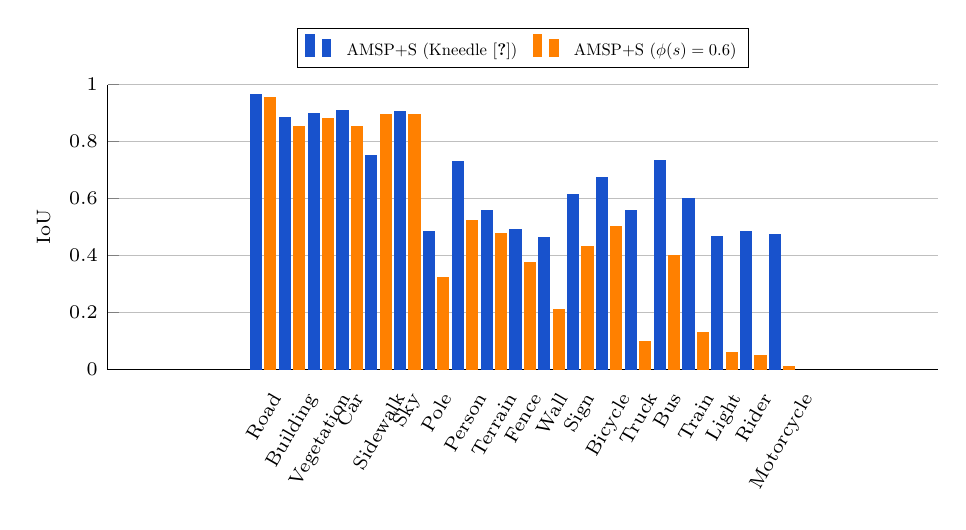
\begin{tikzpicture}
    \begin{axis}[
        width  = \textwidth,
        axis y line*=left,
        symbolic x coords={
            \rotatebox{60}{Road},
            \rotatebox{60}{Building},
            \rotatebox{60}{Vegetation},
            \rotatebox{60}{Car},
            \rotatebox{60}{Sidewalk},
            \rotatebox{60}{Sky},
            \rotatebox{60}{Pole},
            \rotatebox{60}{Person},
            \rotatebox{60}{Terrain},
            \rotatebox{60}{Fence},
            \rotatebox{60}{Wall},
            \rotatebox{60}{Sign},
            \rotatebox{60}{Bicycle},
            \rotatebox{60}{Truck},
            \rotatebox{60}{Bus},
            \rotatebox{60}{Train},
            \rotatebox{60}{Light},
            \rotatebox{60}{Rider},
            \rotatebox{60}{Motorcycle},
        },
        axis x line=bottom,
        height = 5.2cm,
        major x tick style = transparent,
        ybar=3*\pgflinewidth,
        bar width=4pt,
        ymajorgrids = true,
        ylabel = {IoU},
        xtick = data,
        scaled y ticks = false,
        enlarge x limits=0.3,
        axis line style={-},
        ymin=0.0,ymax=1,
        legend columns=2,
        legend cell align=left,
        legend style={
                nodes={scale=0.6},
                at={(0.5,1.2)},
                anchor=north,
                column sep=1ex
        },
        label style={font=\scriptsize},
        tick label style={font=\scriptsize}
    ]
        \addplot[style={cdeepBP,fill=cdeepBP,mark=none}] coordinates {
            (\rotatebox{60}{Road}, 0.964601)
            (\rotatebox{60}{Building}, 0.883573)
            (\rotatebox{60}{Vegetation}, 0.897434)
            (\rotatebox{60}{Car}, 0.908026)
            (\rotatebox{60}{Sidewalk}, 0.750152)
            (\rotatebox{60}{Sky}, 0.906192)
            (\rotatebox{60}{Pole}, 0.482772)
            (\rotatebox{60}{Person}, 0.729143)
            (\rotatebox{60}{Terrain}, 0.55855)
            (\rotatebox{60}{Fence}, 0.492545)
            (\rotatebox{60}{Wall}, 0.461659)
            (\rotatebox{60}{Sign}, 0.614888)
            (\rotatebox{60}{Bicycle}, 0.67332)
            (\rotatebox{60}{Truck}, 0.559177)
            (\rotatebox{60}{Bus}, 0.733037)
            (\rotatebox{60}{Train}, 0.601527)
            (\rotatebox{60}{Light}, 0.468385)
            (\rotatebox{60}{Rider}, 0.483054)
            (\rotatebox{60}{Motorcycle}, 0.473352)
        };
        \addplot[style={orange,fill=orange,mark=none}] coordinates {
            (\rotatebox{60}{Road}, 0.955517)
            (\rotatebox{60}{Building}, 0.852214)
            (\rotatebox{60}{Vegetation}, 0.880035)
            (\rotatebox{60}{Car}, 0.851916)
            (\rotatebox{60}{Sidewalk}, 0.89579)
            (\rotatebox{60}{Sky}, 0.896663)
            (\rotatebox{60}{Pole}, 0.324208)
            (\rotatebox{60}{Person}, 0.523996)
            (\rotatebox{60}{Terrain}, 0.479043)
            (\rotatebox{60}{Fence}, 0.376733)
            (\rotatebox{60}{Wall}, 0.211172)
            (\rotatebox{60}{Sign}, 0.431976)
            (\rotatebox{60}{Bicycle}, 0.503692)
            (\rotatebox{60}{Truck}, 0.097781)
            (\rotatebox{60}{Bus}, 0.401534)
            (\rotatebox{60}{Train}, 0.128532)
            (\rotatebox{60}{Light}, 0.058156)
            (\rotatebox{60}{Rider}, 0.04937)
            (\rotatebox{60}{Motorcycle}, 0.01)
        };
        \legend{AMSP+S (Kneedle \cite{satopaa2011finding}), AMSP+S $( \phi(s) = 0.6 )$}
    \end{axis}
\end{tikzpicture}
\caption{{\em Class-wise IoU according to $\phi(s;\theta)$.} Applying the same $\phi(s)$ of 0.6 to all pixels results in excessive sieving for relatively rare classes, leading to decreased performance for these classes (\eg Light, Rider, and Motorcycle). Based on the ground-truth, class labels are organized in order of the total pixel count for each class.}
\label{fig:sup-class-dist}
\end{figure*}
\begin{figure*}[t!]
    \captionsetup[subfigure]{font=footnotesize}
    \centering
    \begin{subfigure}{.33\linewidth}
        \centering
        \includegraphics[scale=0.322]{Figures/aachen_000000_000019_seg.png}
        \caption{Semantic segmentation}
        \label{subfig:sementic-seg}
    \end{subfigure}
    \begin{subfigure}{.33\linewidth}
        \centering
        \includegraphics[scale=0.322]{Figures/aachen_000000_000019_gt.jpg}
        \caption{Panoptic segmentation}
    \end{subfigure}
    \begin{subfigure}{.33\linewidth}
        \centering
        \includegraphics[scale=0.322]{Figures/aachen_000000_000019_gt_cc.jpg}
        \caption{Oracle superpixels (ours)}
        \label{subfig:oralce-seg}
    \end{subfigure} 
    \caption{{\em Difference between conventional segmentations and oracle superpixels.} (a) When sharing the same class label, they are depicted as identical superpixels (\ie green color on separate trees).  (b) Although a building is divided by a pole, it is represented as a single superpixel (\ie cyan color). (c) We consider a building as two distinct superpixels (\ie cyan and light yellow colors).}
    \label{fig:sup-oracle-superpixels}
\end{figure*}


We provide the reason for introducing 
the threshold function $\phi(s)$
personalized for each superpixel $s$, described in Section \ref{sec:sieving-technique}.
We obtain the dominant label $\text{D}(s)$ for a queried superpixel $s$, however, we only propagate the label to pixels $x \in s$ that are predicted to have a positive impact on the training of model $\theta$ as:
\begin{equation}
h(s;\theta) := \{ x \in s: f_\theta \big( \text{D}(s); x \big) \geq \phi(s; \theta) \} \;,
\end{equation}
where $f_\theta \left( \text{D}(s);x \right)$ implies the confidence of pixel $x$ to dominant label $\text{D}(s)$ given $\theta$ and $\phi(s;\theta)$ determines the degree of sieving.
In Table \ref{tab:sieving}, we study the effect of various $\phi(s;\theta)$.
When the same $\phi(s;\theta)$ is applied to all pixels, it causes class imbalance by leaving relatively easy classes as described in Figure \ref{fig:sup-class-dist}.
To avoid this issue, we utilize the Kneedle algorithm \cite{satopaa2011finding} to obtain different $\phi(s;\theta)$ for each superpixel $s$.
Specifically, $\phi(s; \theta)$ is a knee point of the cumulative distribution function of values of $f_\theta \big( \text{D}(s); x \big)$ in superpixel $x \in s$.
However, for the Kneedle algorithm to work accurately, the curve of cumulative distribution must be either convex or concave. 
In addition, the algorithm may provide inaccurate knee points on very smooth curves.
To address this issue, we use a subset of uniformly sampled values based on $f_\theta(\text{D}(s);x)$, instead of using the distribution for all pixels.
We sample 20 and 5 pixels for Cityscapes and PASCAL datasets, respectively.
In Figure \ref{fig:sup-knee-points}, different knee points are detected according to the dominant class of superpixels.







\begin{figure*}[!ht]
    \captionsetup[subfigure]{font=scriptsize,labelfont=scriptsize,aboveskip=0.05cm,belowskip=-0.15cm}
    \centering
    \hspace{-1mm}
    \begin{subfigure}{.235\linewidth}
        \centering
        \begin{tikzpicture}
            \begin{axis}[
                legend style={nodes={scale=0.35}, at={(0.03, 0.24)}, anchor=west}, 
                xlabel={ASA$(S;G)$},
                ylabel={mIoU (\%)},
                width=1.23\linewidth,
                height=1.23\linewidth,
                ymin=50.8,
                ymax=63.2,
                ytick={51, 53, 55, 57, 59, 61, 63},
                xlabel style={yshift=0.15cm},
                ylabel style={yshift=-0.2cm},
                legend columns=2,
                xmin=0.877,
                xmax=0.971,
                label style={font=\scriptsize},
                tick label style={font=\scriptsize},
                x tick label style={
                    /pgf/number format/.cd,
                        fixed,
                }
            ]
            \addplot[cdeepBP, only marks] table[col sep=comma, x=ASASG, y=mIoU]{Data/correlation_asasg.csv};
            \addplot[very thick, orange] table[col sep=comma, x=ASASG, y={create col/linear regression = {y=mIoU}}
            ]{Data/correlation_asasg.csv};
            \draw (0.5\linewidth, 0.35\linewidth) node {\scriptsize$\text{Corr} = 0.05$};
            \end{axis}
        \end{tikzpicture}
    \end{subfigure}
    \hspace{1mm}
    \begin{subfigure}{.235\linewidth}
        \centering
        \begin{tikzpicture}
            \begin{axis}[
                legend style={nodes={scale=0.35}, at={(0.03, 0.24)}, anchor=west}, 
                xlabel={ASA$(G;S)$},
                ylabel={mIoU (\%)},
                width=1.23\linewidth,
                height=1.23\linewidth,
                ymin=50.8,
                ymax=63.2,
                xlabel style={yshift=0.15cm},
                ylabel style={yshift=-0.2cm},
                ytick={51, 53, 55, 57, 59, 61, 63},
                legend columns=2,
                xmin=-0.05,
                xmax=0.657,
                label style={font=\scriptsize},
                tick label style={font=\scriptsize},
                x tick label style={
                    /pgf/number format/.cd,
                        fixed,
                }
            ]
            \addplot[cdeepBP, only marks] table[col sep=comma, x=ASAGS, y=mIoU]{Data/correlation_asags.csv};
            \addplot[very thick, orange] table[col sep=comma, x=ASAGS, y={create col/linear regression = {y=mIoU}}
            ]{Data/correlation_asags.csv};
            \draw (0.5\linewidth, 0.35\linewidth) node {\scriptsize$\text{Corr}=0.71$};
            \end{axis}
        \end{tikzpicture}
    \end{subfigure}
    \hspace{1mm}
    \begin{subfigure}{.235\linewidth}
        \centering
        \begin{tikzpicture}
            \begin{axis}[
                legend style={nodes={scale=0.35}, at={(0.03, 0.24)}, anchor=west}, 
                xlabel={AP$(S;G)$},
                ylabel={mIoU (\%)},
                width=1.23\linewidth,
                height=1.23\linewidth,
                ymin=50.8,
                ymax=63.2,
                ytick={51, 53, 55, 57, 59, 61, 63},
                xlabel style={yshift=0.15cm},
                ylabel style={yshift=-0.2cm},
                legend columns=2,
                xmin=0.87,
                xmax=0.97,
                label style={font=\scriptsize},
                tick label style={font=\scriptsize},
                x tick label style={
                    /pgf/number format/.cd,
                        fixed,
                }
            ]
            \addplot[cdeepBP, only marks] table[col sep=comma, x=APSG, y=mIoU]{Data/correlation_apsg.csv};
            \addplot[very thick, orange] table[col sep=comma, x=APSG, y={create col/linear regression = {y=mIoU}}
            ]{Data/correlation_apsg.csv};
            \draw (0.5\linewidth, 0.35\linewidth) node {\scriptsize$\text{Corr} = -0.22$};
            \end{axis}
        \end{tikzpicture}
    \end{subfigure}
    \hspace{1mm}
    \begin{subfigure}{.235\linewidth}
        \centering
        \begin{tikzpicture}
            \begin{axis}[
                legend style={nodes={scale=0.35}, at={(0.03, 0.24)}, anchor=west}, 
                xlabel={AR$(S;G)$},
                ylabel={mIoU (\%)},
                width=1.23\linewidth,
                height=1.23\linewidth,
                ymin=50.8,
                ymax=63.2,
                xlabel style={yshift=0.15cm},
                ylabel style={yshift=-0.2cm},
                ytick={51, 53, 55, 57, 59, 61, 63},
                legend columns=2,
                xmin=0,
                xmax=0.057,
                label style={font=\scriptsize},
                tick label style={font=\scriptsize},
                x tick label style={
                    /pgf/number format/.cd,
                        fixed,
                    /tikz/.cd,
                }
            ]
            \addplot[cdeepBP, only marks] table[col sep=comma, x=ARSG, y=mIoU]{Data/correlation_arsg.csv};
            \addplot[very thick, orange] table[col sep=comma, x=ARSG, y={create col/linear regression = {y=mIoU}}
            ]{Data/correlation_arsg.csv};
            \draw (0.5\linewidth, 0.35\linewidth) node {\scriptsize$\text{Corr}=-0.02$};
            \end{axis}
        \end{tikzpicture}
    \end{subfigure}
    \hspace{-5mm}
    \begin{subfigure}{.235\linewidth}
        \centering
        \begin{tikzpicture}
            \begin{axis}[
                legend style={nodes={scale=0.35}, at={(0.03, 0.24)}, anchor=west}, 
                xlabel={AF$(S;G)$},
                ylabel={mIoU (\%)},
                width=1.23\linewidth,
                height=1.23\linewidth,
                ymin=50.8,
                ymax=63.2,
                ytick={51, 53, 55, 57, 59, 61, 63},
                xlabel style={yshift=0.15cm},
                ylabel style={yshift=-0.2cm},
                legend columns=2,
                xmin=0,
                xmax=0.082,
                label style={font=\scriptsize},
                tick label style={font=\scriptsize},
                x tick label style={
                    /pgf/number format/.cd,
                        fixed,
                    /tikz/.cd,
                }
            ]
            \addplot[cdeepBP, only marks] table[col sep=comma, x=AFSG, y=mIoU]{Data/correlation_afsg.csv};
            \addplot[very thick, orange] table[col sep=comma, x=AFSG, y={create col/linear regression = {y=mIoU}}
            ]{Data/correlation_afsg.csv};
            \draw (0.5\linewidth, 0.35\linewidth) node {\scriptsize$\text{Corr} = -0.01$};
            \end{axis}
        \end{tikzpicture}
    \end{subfigure}
    \hspace{1mm}
    \begin{subfigure}{.235\linewidth}
        \centering
        \begin{tikzpicture}
            \begin{axis}[
                legend style={nodes={scale=0.35}, at={(0.03, 0.24)}, anchor=west}, 
                xlabel={AP$(G;S)$},
                ylabel={mIoU (\%)},
                width=1.23\linewidth,
                height=1.23\linewidth,
                ymin=50.8,
                ymax=63.2,
                xlabel style={yshift=0.15cm},
                ylabel style={yshift=-0.2cm},
                ytick={51, 53, 55, 57, 59, 61, 63},
                legend columns=2,
                xmin=0.35,
                xmax=0.74,
                label style={font=\scriptsize},
                tick label style={font=\scriptsize},
                x tick label style={
                    /pgf/number format/.cd,
                        fixed,
                }
            ]
            \addplot[cdeepBP, only marks] table[col sep=comma, x=APGS, y=mIoU]{Data/correlation_apgs.csv};
            \addplot[very thick, orange] table[col sep=comma, x=APGS, y={create col/linear regression = {y=mIoU}}
            ]{Data/correlation_apgs.csv};
            \draw (0.5\linewidth, 0.35\linewidth) node {\scriptsize$\text{Corr}=-0.43$};
            \end{axis}
        \end{tikzpicture}
    \end{subfigure}
    \hspace{1mm}
    \begin{subfigure}{.235\linewidth}
        \centering
        \begin{tikzpicture}
            \begin{axis}[
                legend style={nodes={scale=0.35}, at={(0.03, 0.24)}, anchor=west}, 
                xlabel={AR$(G;S)$},
                ylabel={mIoU (\%)},
                width=1.23\linewidth,
                height=1.23\linewidth,
                ymin=50.8,
                ymax=63.2,
                ytick={51, 53, 55, 57, 59, 61, 63},
                xlabel style={yshift=0.15cm},
                ylabel style={yshift=-0.2cm},
                legend columns=2,
                xmin=0.21,
                xmax=0.696,
                label style={font=\scriptsize},
                tick label style={font=\scriptsize},
                x tick label style={
                    /pgf/number format/.cd,
                        fixed,
                }
            ]
            \addplot[cdeepBP, only marks] table[col sep=comma, x=ARGS, y=mIoU]{Data/correlation_args.csv};
            \addplot[very thick, orange] table[col sep=comma, x=ARGS, y={create col/linear regression = {y=mIoU}}
            ]{Data/correlation_args.csv};
            \draw (0.5\linewidth, 0.35\linewidth) node {\scriptsize$\text{Corr} = 0.57$};
            \end{axis}
        \end{tikzpicture}
    \end{subfigure}
    \hspace{1mm}
    \begin{subfigure}{.235\linewidth}
        \centering
        \begin{tikzpicture}
            \begin{axis}[
                legend style={nodes={scale=0.35}, at={(0.03, 0.24)}, anchor=west}, 
                xlabel={AF$(G;S)$},
                ylabel={mIoU (\%)},
                width=1.23\linewidth,
                height=1.23\linewidth,
                ymin=50.8,
                ymax=63.2,
                xlabel style={yshift=0.15cm},
                ylabel style={yshift=-0.2cm},
                ytick={51, 53, 55, 57, 59, 61, 63},
                legend columns=2,
                xmin=0.173,
                xmax=0.371,
                label style={font=\scriptsize},
                tick label style={font=\scriptsize},
                x tick label style={
                    /pgf/number format/.cd,
                        fixed,
                }
            ]
            \addplot[cdeepBP, only marks] table[col sep=comma, x=AFGS, y=mIoU]{Data/correlation_afgs.csv};
            \addplot[very thick, orange] table[col sep=comma, x=AFGS, y={create col/linear regression = {y=mIoU}}
            ]{Data/correlation_afgs.csv};
            \draw (0.5\linewidth, 0.35\linewidth) node {\scriptsize$\textbf{Corr}=\textbf{0.95}$};
            \end{axis}
        \end{tikzpicture}
    \end{subfigure}
    \caption{{\em Relationship between metrics and mIoU.} The correlation between AF$(G;S)$ and mIoU is especially high. For the correlation calculation, \textit{Oracle} in Table \ref{tab:quantitative} is excluded.}
    \label{fig:sup-correlation}
\end{figure*}
\begin{figure*}[t!]
    \captionsetup[subfigure]{font=footnotesize,labelfont=footnotesize,aboveskip=0.05cm,belowskip=-0.15cm}
    \centering
    \hspace{-1mm}
    \begin{subfigure}{.235\linewidth}
        \centering
        \begin{tikzpicture}
            \begin{axis}[
                legend style={nodes={scale=0.35}, at={(0.03, 0.24)}, anchor=west}, 
                xlabel={AF$(G;S)$},
                ylabel={mIoU (\%)},
                width=1.23\linewidth,
                height=1.23\linewidth,
                ymin=50.8,
                ymax=63.2,
                xlabel style={yshift=0.15cm},
                ylabel style={yshift=-0.2cm},
                ytick={51, 53, 55, 57, 59, 61, 63},
                legend columns=2,
                xmin=0.06,
                xmax=0.42,
                label style={font=\scriptsize},
                tick label style={font=\scriptsize},
                x tick label style={
                    /pgf/number format/.cd,
                        fixed,
                }
            ]
            \addplot[cdeepBP, only marks] table[col sep=comma, x=AFGS, y=mIoU]{Data/correlation_afgs_semantic.csv};
            \addplot[very thick, orange] table[col sep=comma, x=AFGS, y={create col/linear regression = {y=mIoU}}
            ]{Data/correlation_afgs_semantic.csv};
            \draw (0.5\linewidth, 0.35\linewidth) node {\scriptsize $\text{Corr}=0.57$};
            \end{axis}
        \end{tikzpicture}
        \caption{Semantic segmentation}
    \end{subfigure}
    \hspace{1mm}
    \begin{subfigure}{.235\linewidth}
        \centering
        \begin{tikzpicture}
            \begin{axis}[
                legend style={nodes={scale=0.35}, at={(0.03, 0.24)}, anchor=west}, 
                xlabel={AF$(G;S)$},
                ylabel={mIoU (\%)},
                width=1.23\linewidth,
                height=1.23\linewidth,
                ymin=50.8,
                ymax=63.2,
                xlabel style={yshift=0.15cm},
                ylabel style={yshift=-0.2cm},
                ytick={51, 53, 55, 57, 59, 61, 63},
                legend columns=2,
                xmin=0.21,
                xmax=0.39,
                label style={font=\scriptsize},
                tick label style={font=\scriptsize},
                x tick label style={
                    /pgf/number format/.cd,
                        fixed,
                }
            ]
            \addplot[cdeepBP, only marks] table[col sep=comma, x=AFGS, y=mIoU]{Data/correlation_afgs_panoptic.csv};
            \addplot[very thick, orange] table[col sep=comma, x=AFGS, y={create col/linear regression = {y=mIoU}}
            ]{Data/correlation_afgs_panoptic.csv};
            \draw (0.5\linewidth, 0.35\linewidth) node {\scriptsize$\textbf{Corr}=\textbf{0.95}$};
            \end{axis}
        \end{tikzpicture}
        \caption{Panoptic segmentation}
    \end{subfigure}
    \hspace{1mm}
    \begin{subfigure}{.235\linewidth}
        \centering
        \begin{tikzpicture}
            \begin{axis}[
                legend style={nodes={scale=0.35}, at={(0.03, 0.24)}, anchor=west}, 
                xlabel={AF$(G;S)$},
                ylabel={mIoU (\%)},
                width=1.23\linewidth,
                height=1.23\linewidth,
                ymin=50.8,
                ymax=63.2,
                xlabel style={yshift=0.15cm},
                ylabel style={yshift=-0.2cm},
                ytick={51, 53, 55, 57, 59, 61, 63},
                legend columns=2,
                xmin=0.173,
                xmax=0.371,
                label style={font=\scriptsize},
                tick label style={font=\scriptsize},
                x tick label style={
                    /pgf/number format/.cd,
                        fixed,
                }
            ]
            \addplot[cdeepBP, only marks] table[col sep=comma, x=AFGS, y=mIoU]{Data/correlation_afgs.csv};
            \addplot[very thick, orange] table[col sep=comma, x=AFGS, y={create col/linear regression = {y=mIoU}}
            ]{Data/correlation_afgs.csv};
            \draw (0.5\linewidth, 0.35\linewidth) node {\scriptsize$\textbf{Corr}=\textbf{0.95}$};
            \end{axis}
        \end{tikzpicture}
        \caption{Oracle superpixels}
    \end{subfigure}
    \caption{{\em Relationship between AF$(G;S)$ and mIoU varying $G$.} AF$(G;S)$ and mIoU exhibit a high correlation when ground-truth $G$ is represented by the panoptic segmentation and oracle superpixels in Figure \ref{fig:sup-oracle-superpixels}. For the correlation calculation, \textit{Oracle} in Table \ref{tab:quantitative} is excluded.}
    \label{fig:sup-afgs-g}
\end{figure*}


\begin{figure*}[t!]
    \captionsetup[subfigure]{font=footnotesize}
    \centering
    \begin{subfigure}[!ht]{.245\linewidth}
        \centering
        \includegraphics[scale=0.238]{Figures/fig13_round/bochum_000000_025833_r1.png}
    \end{subfigure}
    \begin{subfigure}[!ht]{.245\linewidth}
        \centering
        \includegraphics[scale=0.238]{Figures/fig13_round/bochum_000000_025833_r2.png}
    \end{subfigure}
    \begin{subfigure}[!ht]{.245\linewidth}
        \centering
        \includegraphics[scale=0.238]{Figures/fig13_round/bochum_000000_025833_r3.png}
    \end{subfigure}
    \begin{subfigure}[!ht]{.245\linewidth}
        \centering
        \includegraphics[scale=0.238]{Figures/fig13_round/bochum_000000_025833_r4.png}
    \end{subfigure}

    
    \begin{subfigure}[!ht]{.245\linewidth}
        \centering
        \includegraphics[scale=0.238]{Figures/fig13_round/hanover_000000_058189_r1.png}
    \end{subfigure}
    \begin{subfigure}[!ht]{.245\linewidth}
        \centering
        \includegraphics[scale=0.238]{Figures/fig13_round/hanover_000000_058189_r2.png}
    \end{subfigure}
    \begin{subfigure}[!ht]{.245\linewidth}
        \centering
        \includegraphics[scale=0.238]{Figures/fig13_round/hanover_000000_058189_r3.png}
    \end{subfigure}
    \begin{subfigure}[!ht]{.245\linewidth}
        \centering
        \includegraphics[scale=0.238]{Figures/fig13_round/hanover_000000_058189_r4.png}
    \end{subfigure}
    
    
    \begin{subfigure}[!ht]{.245\linewidth}
        \centering
        \includegraphics[scale=0.238]{Figures/fig13_round/zurich_000117_000019_r1.png}
        \caption{Adaptive merged $(t=1)$}
    \end{subfigure}
    \begin{subfigure}[!ht]{.245\linewidth}
        \centering
        \includegraphics[scale=0.238]{Figures/fig13_round/zurich_000117_000019_r2.png}
        \caption{Adaptive merged $(t=2)$}
    \end{subfigure}
    \begin{subfigure}[!ht]{.245\linewidth}
        \centering
        \includegraphics[scale=0.238]{Figures/fig13_round/zurich_000117_000019_r3.png}
        \caption{Adaptive merged $(t=3)$}
    \end{subfigure}
    \begin{subfigure}[!ht]{.245\linewidth}
        \centering
        \includegraphics[scale=0.238]{Figures/fig13_round/zurich_000117_000019_r4.png}
        \caption{Adaptive merged $(t=4)$}
    \end{subfigure}
    \caption{{\em Qualitative results with varying round.}
    (a-d) Superpixels generated with proposed adaptive merging at rounds 1 to 4.
    Thanks to the improved model, we observe that the merging becomes more accurate as the round increases. We use the model reported in Figure~\ref{fig:(a)-effect}.}
    \label{fig:sup-round}
    \vspace{-2mm}
\end{figure*}


\begin{figure*}[t!]
    \captionsetup[subfigure]{font=footnotesize}
    \centering
    \begin{subfigure}[!ht]{.245\linewidth}
        \centering
        \includegraphics[scale=0.238]{Figures/fig14_eps/bremen_000310_000019_00.png}
    \end{subfigure}
    \begin{subfigure}[!ht]{.245\linewidth}
        \centering
        \includegraphics[scale=0.238]{Figures/fig14_eps/bremen_000310_000019_01.png}
    \end{subfigure}
    \begin{subfigure}[!ht]{.245\linewidth}
        \centering
        \includegraphics[scale=0.238]{Figures/fig14_eps/bremen_000310_000019_015.png}
    \end{subfigure}
    \begin{subfigure}[!ht]{.245\linewidth}
        \centering
        \includegraphics[scale=0.238]{Figures/fig14_eps/bremen_000310_000019_02.png}
    \end{subfigure}

    
    \begin{subfigure}[!ht]{.245\linewidth}
        \centering
        \includegraphics[scale=0.238]{Figures/fig14_eps/zurich_000012_000019_005.png}
    \end{subfigure}
    \begin{subfigure}[!ht]{.245\linewidth}
        \centering
        \includegraphics[scale=0.238]{Figures/fig14_eps/zurich_000012_000019_01.png}
    \end{subfigure}
    \begin{subfigure}[!ht]{.245\linewidth}
        \centering
        \includegraphics[scale=0.238]{Figures/fig14_eps/zurich_000012_000019_015.png}
    \end{subfigure}
    \begin{subfigure}[!ht]{.245\linewidth}
        \centering
        \includegraphics[scale=0.238]{Figures/fig14_eps/zurich_000012_000019_02.png}
    \end{subfigure}
    
    
    \begin{subfigure}[!ht]{.245\linewidth}
        \centering
        \includegraphics[scale=0.238]{Figures/fig14_eps/zurich_000036_000019_005.png}
        \caption{Adaptive merged $(\epsilon=0.05)$}
    \end{subfigure}
    \begin{subfigure}[!ht]{.245\linewidth}
        \centering
        \includegraphics[scale=0.238]{Figures/fig14_eps/zurich_000036_000019_01.png}
        \caption{Adaptive merged $(\epsilon=0.1)$}
    \end{subfigure}
    \begin{subfigure}[!ht]{.245\linewidth}
        \centering
        \includegraphics[scale=0.238]{Figures/fig14_eps/zurich_000036_000019_015.png}
        \caption{Adaptive merged $(\epsilon=0.15)$}
    \end{subfigure}
    \begin{subfigure}[!ht]{.245\linewidth}
        \centering
        \includegraphics[scale=0.238]{Figures/fig14_eps/zurich_000036_000019_02.png}
        \caption{Adaptive merged $(\epsilon=0.2)$}
    \end{subfigure}
    \caption{{\em Qualitative results with varying $\epsilon$.}
    (a-d) Superpixels are generated with proposed adaptive merging with $\epsilon$: 0.05, 0.1, 0.15, 0.2. %
    We observe that an increase in $\epsilon$ gives more aggressive merging. Merging is conducted on Cityscapes with a base superpixel size of 256. }
    \label{fig:sup-epsilon}
    \vspace{-3mm}
\end{figure*}
\begin{figure*}[t!]
    \captionsetup[subfigure]{font=footnotesize}
    \centering
    \begin{subfigure}{.33\linewidth}
        \centering
        \includegraphics[scale=0.322]{Figures/fig12_qual/fig_12_1a.png}
    \end{subfigure}
    \begin{subfigure}{.33\linewidth}
        \centering
        \includegraphics[scale=0.322]{Figures/fig12_qual/fig_12_1b.png}
    \end{subfigure}
    \begin{subfigure}{.33\linewidth}
        \centering
        \includegraphics[scale=0.322]{Figures/fig12_qual/fig_12_1c_n.png}
    \end{subfigure}

    
    \begin{subfigure}{.33\linewidth}
        \centering
        \includegraphics[scale=0.322]{Figures/fig12_qual/fig_12_2a.png}
    \end{subfigure}
    \begin{subfigure}{.33\linewidth}
        \centering
        \includegraphics[scale=0.322]{Figures/fig12_qual/fig_12_2b.png}
    \end{subfigure}
    \begin{subfigure}{.33\linewidth}
        \centering
        \includegraphics[scale=0.322]{Figures/fig12_qual/fig_12_2c_n.png}
    \end{subfigure}

    \begin{subfigure}{.33\linewidth}
        \centering
        \includegraphics[scale=0.322]{Figures/fig12_qual/fig_12_3a.png}
        \caption{Base superpixels~\cite{van2012seeds}}
    \end{subfigure}
    \begin{subfigure}{.33\linewidth}
        \centering
        \includegraphics[scale=0.322]{Figures/fig12_qual/fig_12_3b.png}
        \caption{Merged superpixels (Ours)}
    \end{subfigure}
    \begin{subfigure}{.33\linewidth}
        \centering
        \includegraphics[scale=0.322]{Figures/fig12_qual/fig_12_3c_n.png}
        \caption{Oracle superpixels}
    \end{subfigure}
    \caption{{\em Qualitative results of adaptive superpixels.} (a) Base superpixel generated by SEEDS~\cite{van2012seeds} with size 256. (b) Superpixels generated with proposed adaptive merging at round 4. (c) Oracle superpixels generated from the ground truth.}
    \label{fig:sup-same-paper}
    \vspace{3mm}
\end{figure*}

\section{Further discussion on the oracle superpixels}
\label{fig:sup-oracle}

In Section \ref{para:oracle-superpixels},
we introduce the oracle superpixels,
which we believe is an achievable optimal set of superpixels for active learning.
For clarification,  
we provide the detailed process of generating the proposed oracle superpixels.
In addition, we provide further insights
into the achievable notion of optimal superpixels.

The Cityscapes dataset is equipped with the ground-truth annotations for semantic segmentation, represented by dense pixel-wise labels: \ie., each pixel in an annotated image is assigned an ID that represents a ground-truth semantic category~(Figure~\ref{subfig:sementic-seg}). In such annotation, each group of pixels that share the same ID aligns perfectly with the boundary of semantic objects. However, each such group is not guaranteed to be a single-connected component of pixels.
For example, different cars in Figure~\ref{subfig:sementic-seg} are assigned the same blue color despite being physically separated, and a car divided into two parts due to an obstructing pole is still colored blue. 
This is opposed to what we hope to achieve by merging two adjacent superpixels repeatedly.
To address this issue, we subdivide each superpixel as necessary to ensure that every pixel within a superpixel is adjacent to each other.
We utilize OpenCV~\cite{opencv_library} and Shapely~\cite{shapely2007} to identify the maximal connected component of pixels sharing the same semantic. 
We apply the same procedure to annotated images in the PASCAL dataset
Figure~\ref{fig:sup-oracle-superpixels} illustrates the distinction between conventional semantic and panoptic segmentation and our oracle superpixels.

The Cityscapes and PASCAL datasets are divided into 327k and 16k oracle superpixels, respectively.
It is worth noting that the PASCAL has a lower number of oracle superpixels due to the smaller number of classes per image.
In other words, only a few objects are of interest in each image, and the rest are simply treated as the background.

\newpage
\section{Further discussion on the achievable metrics}
\label{fig:sup-metrics}



In Table \ref{tab:quantitative}, we evaluate various superpixels using eight metrics with oracle superpixels as ground-truth $G$.
Figure \ref{fig:sup-correlation} shows the correlation between each metric and mIoU. 
We observe that our AF$(G;S)$ can be utilized to look-ahead a model's performance in active learning without training. 
In addition, we examine how different ground-truth $G$ impacts AF$(G;S)$.
In the field of semantic segmentation, two conventional segmentations, semantic and panoptic segmentations in Figure \ref{fig:sup-oracle-superpixels}, are widely used as ground-truth.
Figure \ref{fig:sup-afgs-g} indicates that using panoptic segmentation and oracle superpixels for $G$ results in higher correlation between AF$(G;S)$ and mIoU than semantic segmentation.
However, obtaining panoptic segmentation requires more costs than semantic segmentation since it utilizes additional instance information.
It is worth noting that our oracle superpixels (Figure \ref{subfig:oralce-seg}) can be easily generated even in cost-limited practical situations as they are produced from semantic segmentation (Figure \ref{subfig:sementic-seg}).




\newpage
\section{Additional qualitative adaptive superpixels}
\label{fig:sup-qual}
To facilitate comprehension of the merged superpixels, we display superpixels generated across diverse settings.
The appearance of merged superpixels is mainly determined by the model's performance and $\epsilon$. 
Figure \ref{fig:sup-round} highlights that as the round progresses, the model's performance improves, leading to more accurate merging. 
With the model fixed at round 4, Figure \ref{fig:sup-epsilon} shows the impact of adjusting $\epsilon$.
As $\epsilon$ grows, the merging process intensifies, ultimately decreasing the overall number of superpixels.
In addition, Figure \ref{fig:sup-same-paper} shows further examples of our merged superpixels.







\clearpage
\begin{table*}[t!]
\centering
\setlength\tabcolsep{6pt}
\begin{tabular}{c|l}
\toprule
Notations & Description \\ \midrule
$\mathcal{I}$ & the set of unlabeled images \\ \midrule
$\mathcal{C}$ & the set of class labels \\ \midrule
$t$ & a round \\ \midrule
$x$ & a pixel \\ \midrule
$s$ & a superpixel \\ \midrule
$S_t(i)$ & the set of superpixels in an image $i$ in round $t$ \\ \midrule
$\mathcal{S}_t$ & the set of superpixels in all images in round $t$, $\mathcal{S}_t := \bigcup_{i \in \mathcal{I}} S_t(i)$ \\ \midrule
$B$ & the query budget per round \\ \midrule
$\mathcal{B}_t$ & the set of $B$ selected superpixels in round $t$, $B_t \subset \mathcal{S}_t, |B_t| = B$\\ \midrule
$\theta_t$ & the model at the end of round $t$ \\ \midrule
$y_\theta(x)$ & the estimated dominant label of pixel $x$ given $\theta$ \\ \midrule
$\text{D}(s)$ & the true dominant label of superpixel $s$ \\ \midrule
$\text{D}_\theta(s)$ & the estimated dominant label of superpixel $s$ given $\theta$ \\ \midrule
\multirow{2}{*}{$\mathcal{G}(S) := (S, \mathcal{E}(S))$} & the graph consisting of the superpixels in $S$ as nodes and
the edge set $\mathcal{E}(S)$ \\
& such that $(s, n) \in \mathcal{E}(S)$ for each pair of adjacent superpixels $s, n \in S$.  \\ \midrule
$\epsilon$      & the hyperparameter for merging in \eqref{eq:jsd} \\
\bottomrule
\end{tabular}
\caption{{\em Notations.} The notations used in the paper are defined.}
\label{tab:notations}
\end{table*}




\end{document}
